% This text is proprietary.
% It's a part of presentation made by myself.
% It may not used commercial.
% The noncommercial use such as private and study is free
% Sep. 2005 
% Author: Sascha Frank 
% University Freiburg 
% www.informatik.uni-freiburg.de/~frank/


\documentclass{beamer}

\usetheme{Berlin}

\newcommand{\Rn}{\mathbb R ^ {n}}
\newcommand{\xk}{{{x}^{(k)}}}
\newcommand{\dk}{{\Delta_k}}
\newcommand{\mk}{{m_f}}
\newcommand{\fk}{{f_k}}
\newcommand{\fgk}{{g^{(k)}_f}}
\newcommand{\fhk}{{H^{(k)}_f}}
\newcommand{\ck}{{c^{(k)}_{i}(\xk)}}
\newcommand{\cgk}{{g^{(k)}_{c_i}}}
\newcommand{\mck}{{m_{c_i}}}
\newcommand{\bk}{{B_{\infty}(\xk, \dk)}}
\newcommand{\feasible}{\mathcal F}
\newcommand{\feasiblek}{\mathcal F^{(k)}}
\newcommand{\proj}{\textbf{P}}
\newcommand{\neggrad}{d^{(k)}}


\DeclareMathOperator*{\argmin}{arg\,min}

\usepackage{color}
\usepackage{amsmath}
\usepackage{cancel}
\usepackage{ulem}


\begin{document}


\title{Model-Based Derivative-Free Optimization with Unrelaxable Constraints}   
\author{Trever Hallock} 
\date{\today} 

\frame{\titlepage} 

\section{Introduction}

\begin{frame}{Introduction}
	\begin{itemize}
		\item We develop an algorithm to find local optima of constrained problems
		\item Derivatives not available, only function values
		\item This algorithm is designed for problems with unrelaxable constraints
		\begin{block}{Unrelaxable Constraints}
			Function values are unavailable for infeasible points
		\end{block}
	\end{itemize}
\end{frame}


\begin{frame}{Derivative Free Problem Formulation}
\begin{center}
\label{Problem}
\begin{align*}
\min_x & \quad f(x) \\
  c_i(x) \le 0   & \quad \forall \; 1 \le i \le m \\
\end{align*}
\end{center}
	\begin{itemize}
		\item All functions are black-box functions, meaning that we have no information about their derivatives
		\item For example, optimization problems where the objective or some of the constraints depend on an expensive simulation
		\item Function values may not be available outside of the feasible region, 
		we call these \emph{unrelaxable} constraints
%		\item $S(x)$ is a black-box function, meaning that we have no information about its derivatives
%		\item We assume that $f$ and $c$ are apriori functions
%		 \item We assume the level sets of $f$ are bounded
%		 \item We assume $f$, $c$ are continuously twice differentiable
%		 \item The goal of my research is to develop algorithms for this problem
	\end{itemize}
\end{frame}


\begin{frame}{Applications}
	Problems can arise several different ways:
	\begin{itemize}
		\setlength\itemsep{1.5em}
		\item Physical models are not meaningful for certain inputs
		\begin{itemize}
			\item A simulation quantity represents a concentration level
			\item Well rates in groundwater problems
			\item When decision variables must be ordered
		\end{itemize}
		\item Simulations may not converge
		\begin{itemize}
			\item Inverse Transport Problem \cite{Armstrong}
		\end{itemize}
	\end{itemize}
\end{frame}


\begin{frame}{Why are Unrelaxable Constraints Hard?}
	Building accurate models is harder
	\begin{itemize}
		\item Models require feasible sample points:
	\end{itemize}
	\begin{center}
		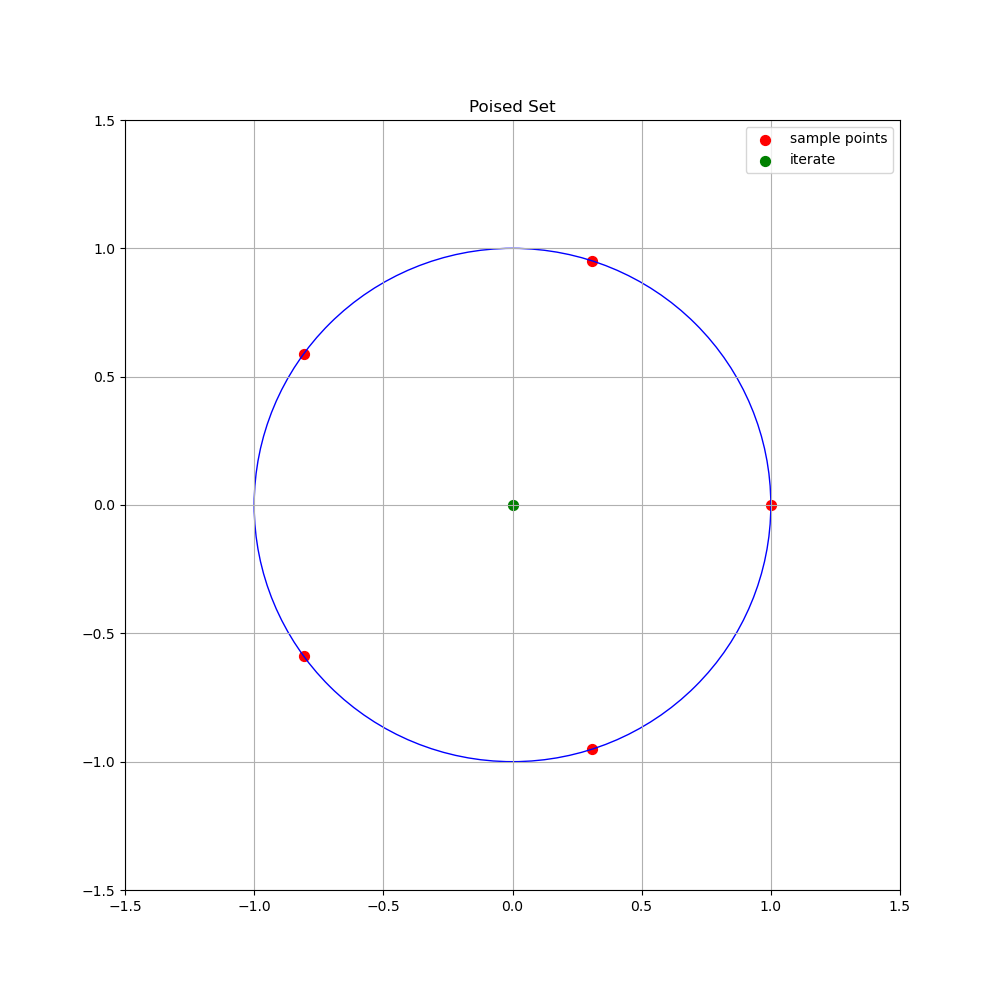
\includegraphics[width=125px]{images/poised.png}
		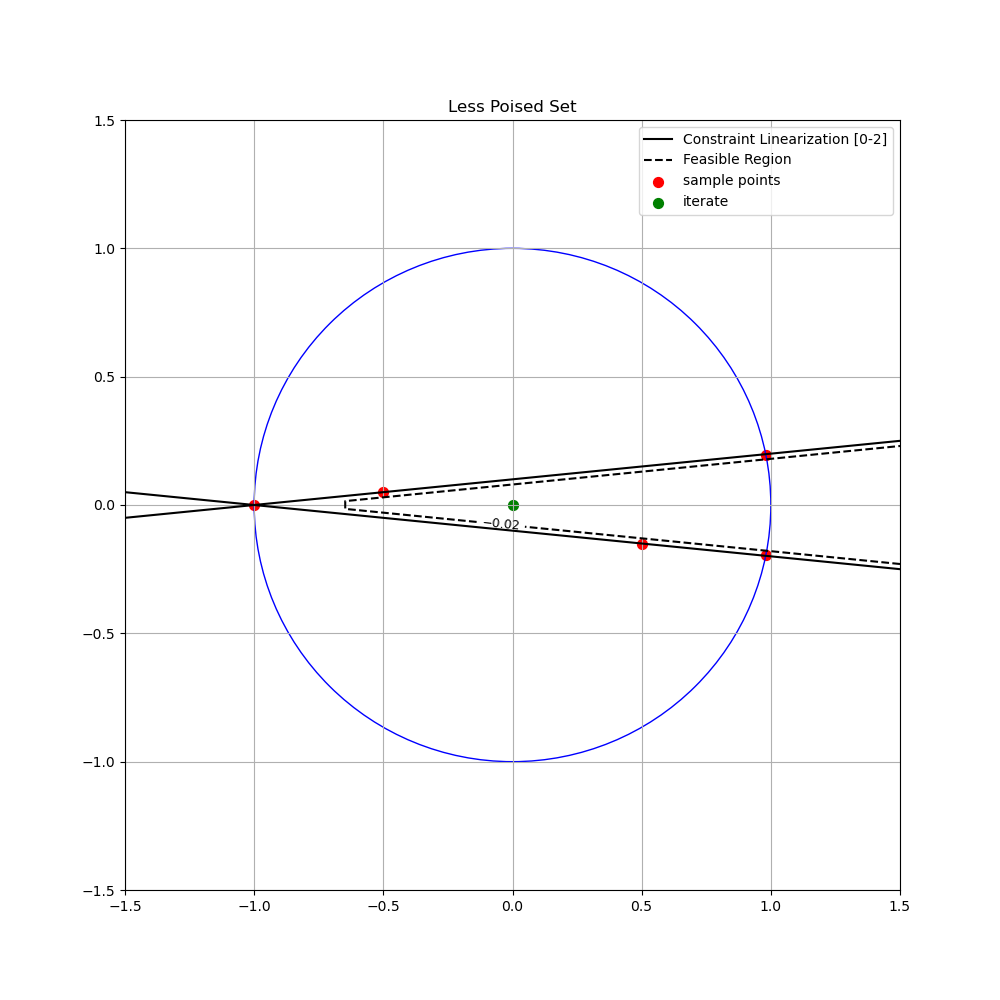
\includegraphics[width=125px]{images/not_poised.png}
	\end{center}
\end{frame}

\begin{frame}{Why are Unrelaxable Constraints Hard?}
	Constraint boundaries are uncertain
	\begin{itemize}
		\item Infeasible function calls are wasteful... How do we avoid them?
	\end{itemize}
	\begin{center}
		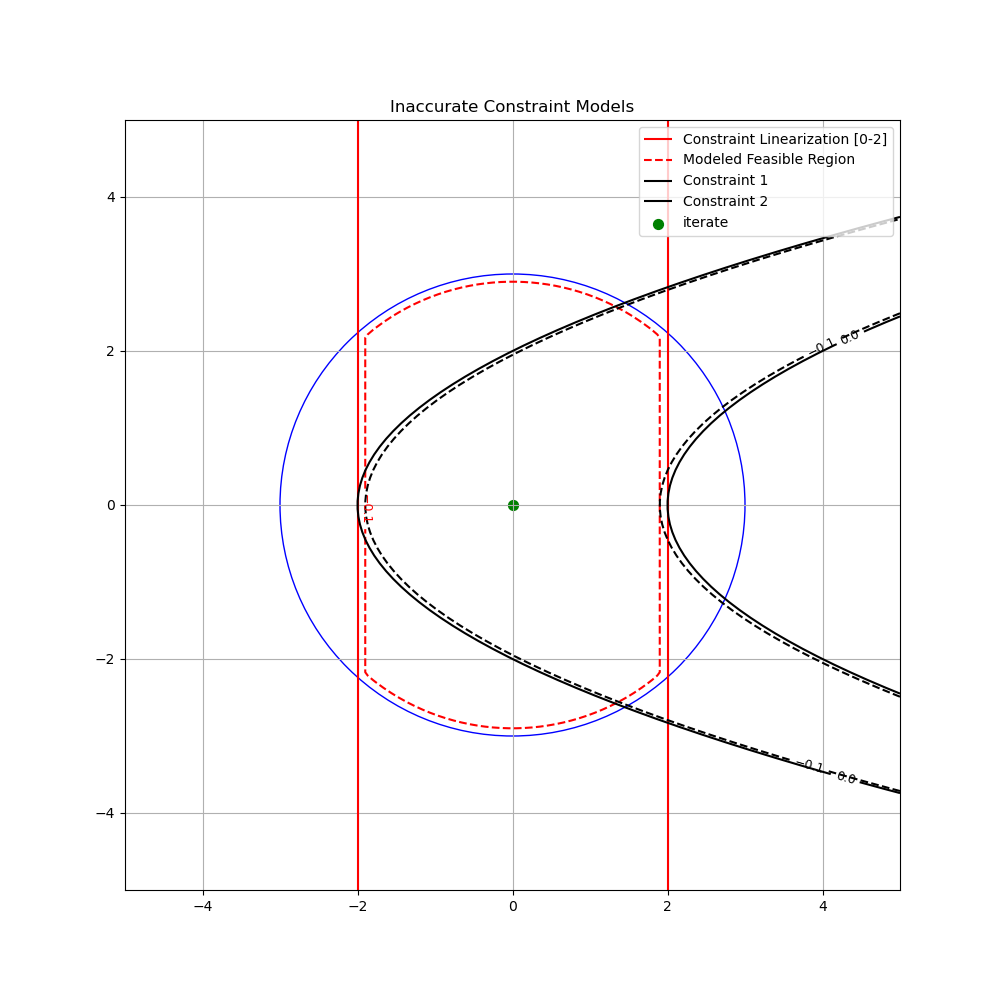
\includegraphics[width=125px]{images/modeled_constraints.png}
	\end{center}
\end{frame}


\frame{\frametitle{Table of Contents}\tableofcontents} 


\section{Derivative Free Background}


\begin{frame}{Model-Based Trust Region Methods}
	\begin{itemize}
		\item[Step 1] \textbf{Construct a model for the current point} \\
			Choose sample points to construct a model
		\item[Step 2] \textbf{Check optimality.} \\
			Compute $\chi\left(\xk\right)$ and compare to a threshold
		\item[Step 3] \textbf{Compute the trial step, and evaluate} \\
			Solve the trust region subproblem using the model functions
		\item[Step 4] \textbf{Check reduction and update radius} \\
			If little progress was made, decrease the trust region radius. \\
			Otherwise, set the next iterate to the trial point
	\end{itemize}
\end{frame}


\begin{frame}{Model Based Trust Region Methods}
	\begin{itemize}
		\item Approximate derivatives of $f$ and $c$ using model functions created from a sample set
		\item We approximate $f$ using a second order model, meaning that we approximate:
		\begin{itemize}
			\item $\mk(x) = \fk + \left(x - \xk \right)^T\fgk + \frac 1 2 \left(x - \xk \right)^T\fhk\left(x - \xk \right) \approx f(x)$
			\item $\fhk \approx \nabla ^2 f(\xk)$
			\item $\fgk \approx \nabla f(\xk)$
			\item $\cgk \approx \nabla c_i(\xk)$
			\item $\mck(x) = \ck + \left(x - \xk\right)^T \cgk \approx c_i(x)$
		\end{itemize}
		\item The model's accuracy depends on the sample points chosen
	\end{itemize}
\end{frame}


\begin{frame}{Geometry of the Sample Set}
	\begin{itemize}
		\item<1, 2, 3> Geometry refers to the relative positions of the sample set of sample points
		\item<1, 2, 3> When the points are not ``well poised", the constructed model can be innacurate \\
		\only<2>{
			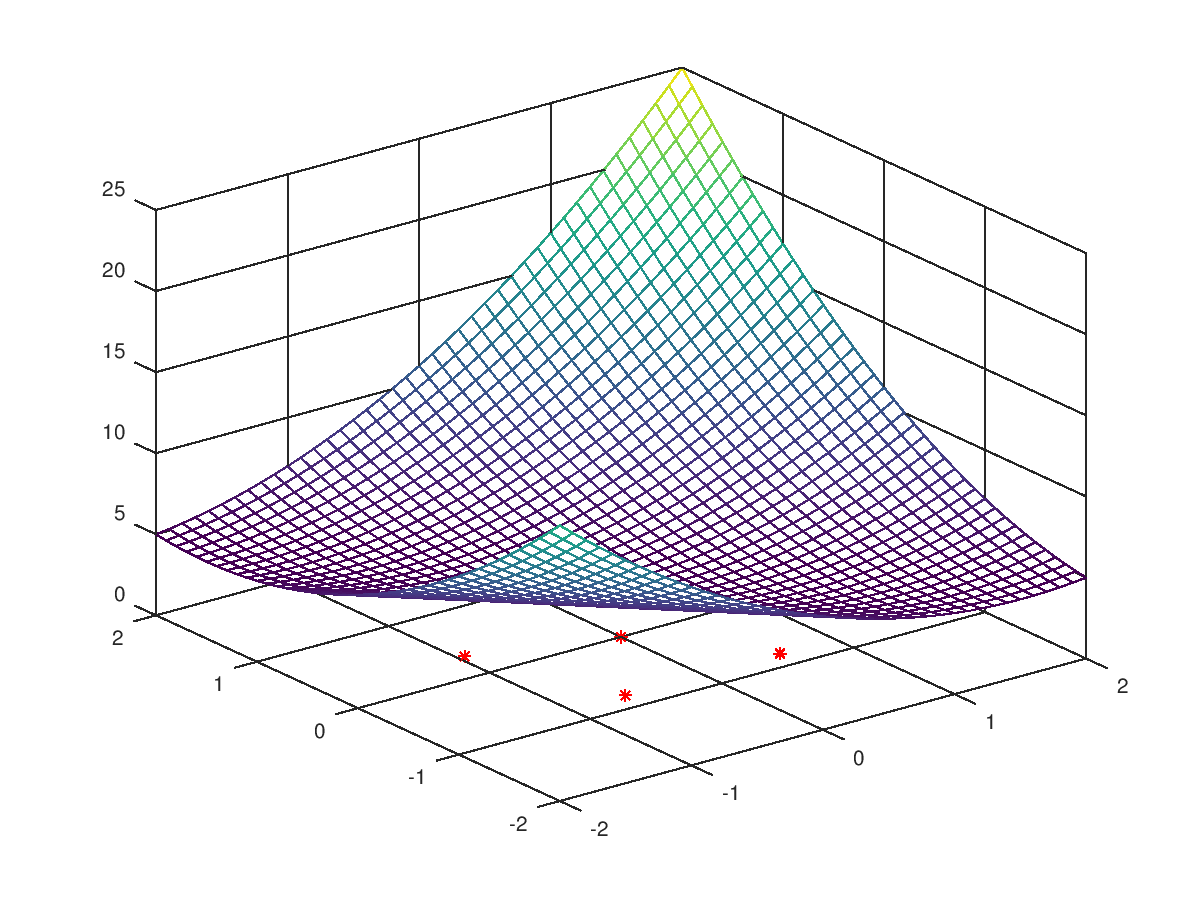
\includegraphics[width=120px]{images/poised_good.png} 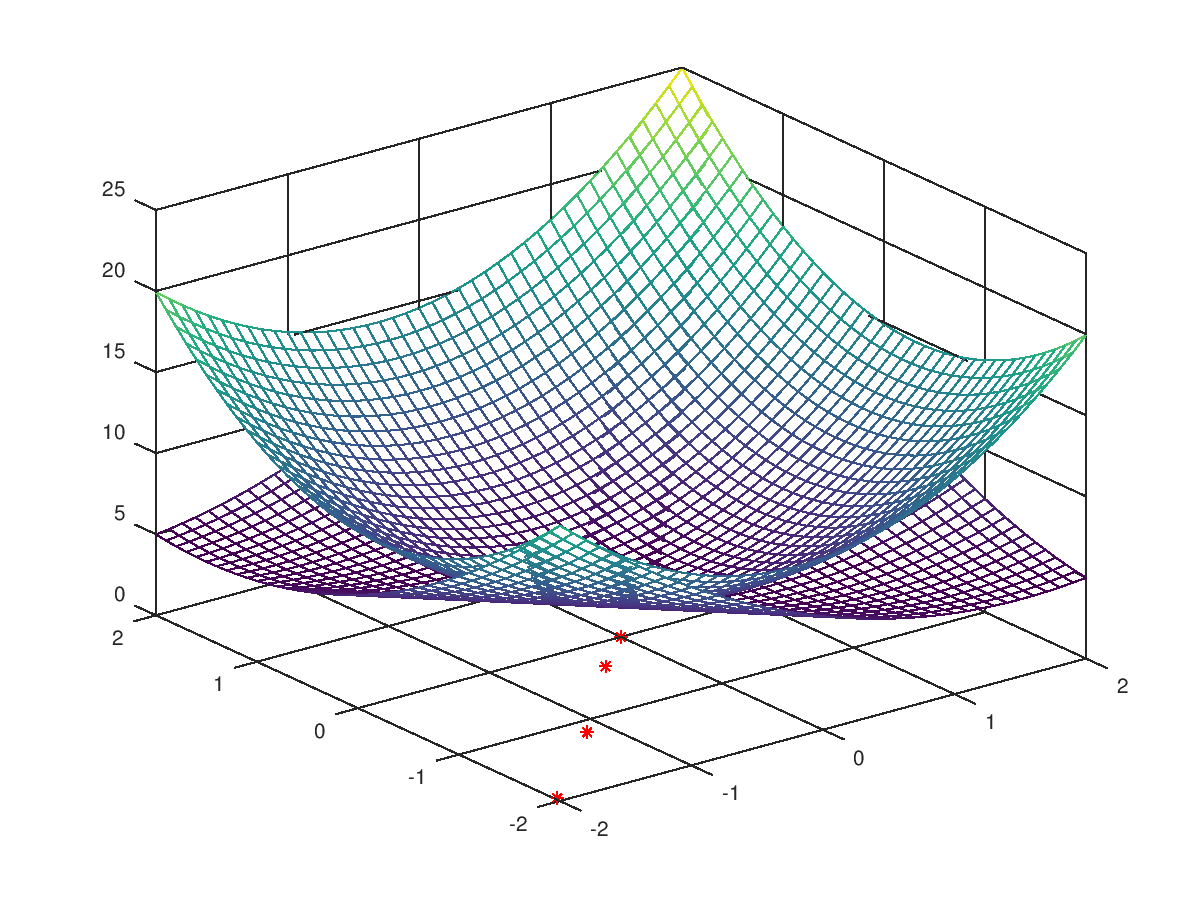
\includegraphics[width=120px]{images/poised_bad.png}
		}
		\item<3> Constructing poised sets over ellipses is well known
		\item<3> Constraints limit what points are available for the sample set
		\item<3> With narrow constraints, well poised sets may not exist
		\only<3>{
			\begin{center}
				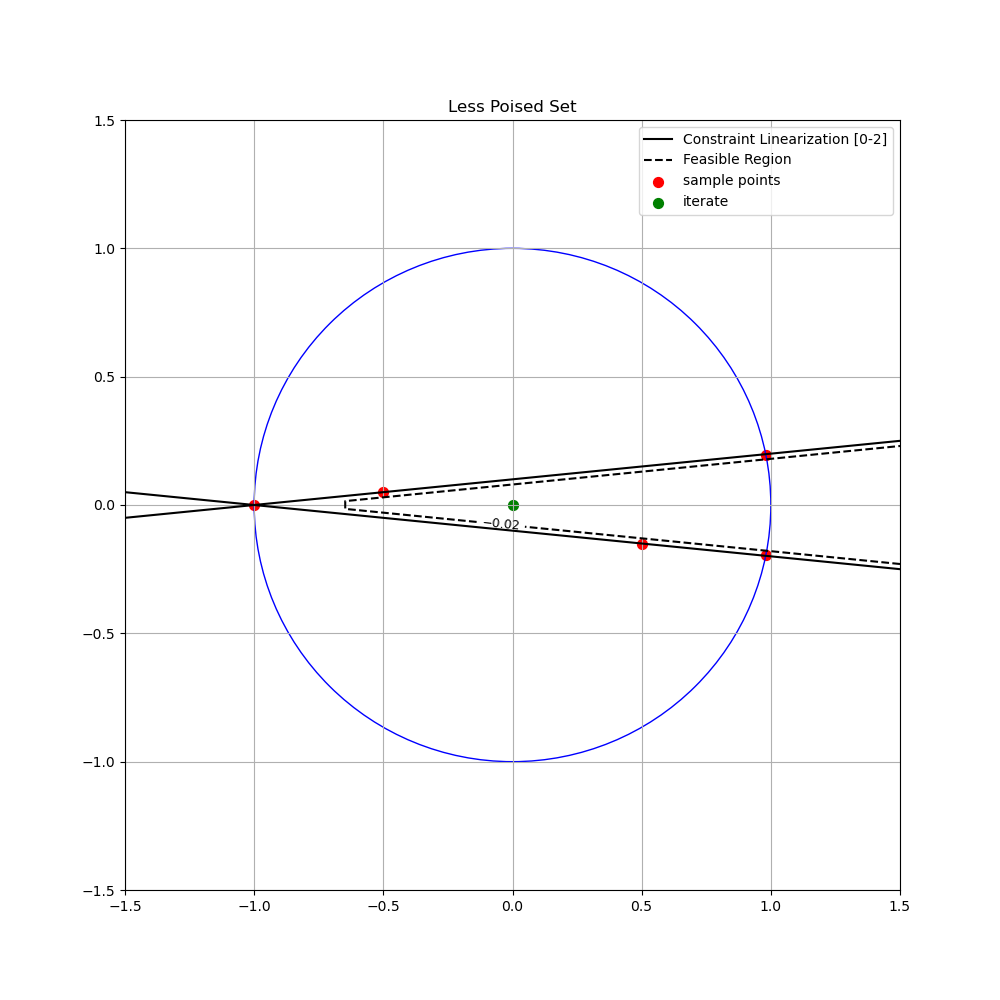
\includegraphics[width=75px]{images/not_poised.png}
			\end{center}
		}
	\end{itemize}
\end{frame}


\begin{frame}{Stopping Conditions}
	\begin{itemize}
% 		\item We had to modify the convergence analysis in a few significant ways
		\item The criticality measure $\chi\left(x\right)$ measures how close to optimality a point $x$ may be
% 		\item One of these was within the criticality measure, $\chi(x)$
		\item If $x$ satisfies the first order necessary conditions for optimality, then $\chi(x) = 0$
		\item We show that $\chi^{(k)} = \chi\left(\xk\right)$ converges to zero
		\item We use the projection of the negative gradient onto the constraints
			$\chi^{(k)} = $
	\end{itemize}
	\begin{center}
		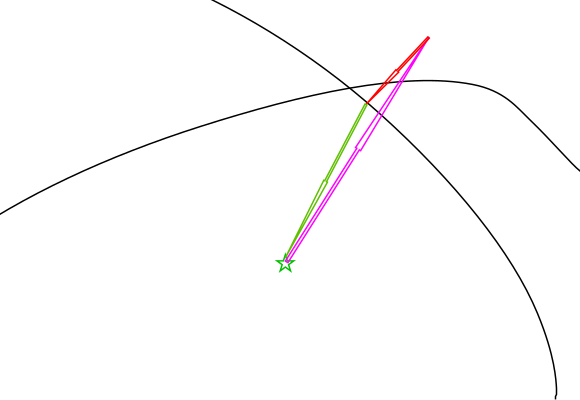
\includegraphics[width=100px]{images/criticality.png}
	\end{center}
\end{frame}

\begin{frame}{Trust Region Subproblem}
	\begin{itemize}
		\item In each iteration, we attempt to solve the trust region subproblem to compute a step direction $s$

		\begin{displaymath}
\begin{array}{lrcc}
min_s & \mk(\xk + s)   &	 &			\\
s.t.  &  \mck(\xk + s) & \le & 0   \quad \forall \; 1 \le i \le m	   \\
	  &  s & \in & B_{\infty}(0, \dk).  \\
\end{array}
		\end{displaymath}
		\item Replaced true functions with model functions
		\item Added trust region constraint
		\item The solution is then used as a trial point for the next iterate
	\end{itemize}
\end{frame}

% % Remove this picture
% \begin{frame}{Model Fitting}
% % 	\begin{align*}
% % 		l_1(x) = -(x-1)(x+1), \;
% % 		l_2(x) = \frac 1 2 x(x+1), \;
% % 		l_3(x) = \frac 1 2 x(x-1) \\
% % 		f(x) = 3 + \sin(x) \quad
% % 		m_f(x) = f(0)l_1(x) + f(1)l_2(x) + f(-1)l_3(x)
% % 	\end{align*}
% 	\begin{center}
% 		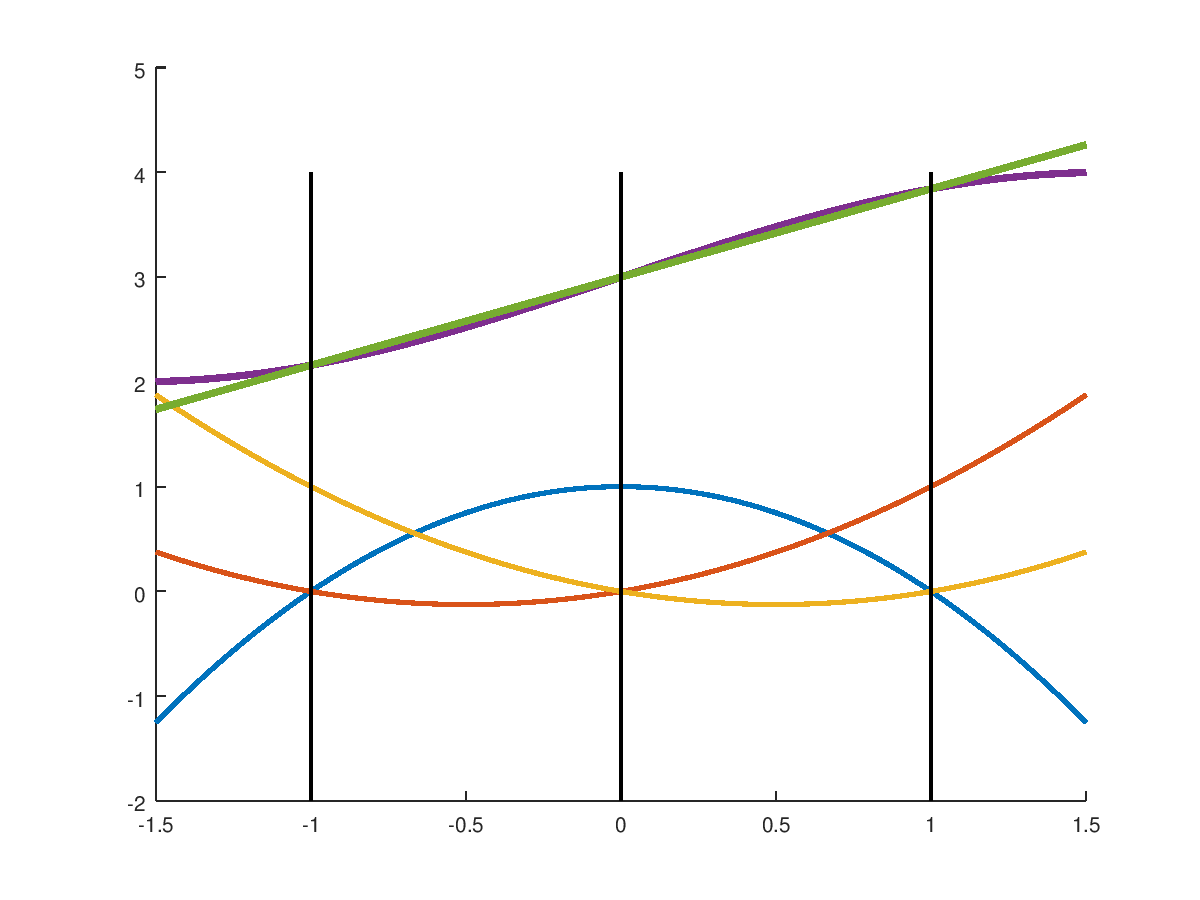
\includegraphics[width=250px]{images/lagrange_polynomials.png}
% 	\end{center}
% \end{frame}


\begin{frame}{Evaluating the trial point}
	\begin{itemize}
		\item After evaluating, we check if the trial point produced enough reduction
		\item One quantity to measure the model's accuracy and the trial points reduction is
\begin{align*}
	\rho_k = \frac{f\left(\xk\right) - f\left(\xk+s^{(k)}\right)}
		{m_k\left(\xk\right) - m_k\left(\xk+s^{(k)}\right)}
\end{align*}
% 		\item Derivative Free Algorithms require the trust region to go to zero
% 		\item Helps determine new trust region radius
		\begin{itemize}
			\item If $\rho_k$ is small, $x^{(k+1)}=\xk$ (reject) and decrease radius
			\item If $\rho_k$ is intermediate, $x^{(k+1)}=\xk+s^{(k)}$ (accept) and decrease radius
			\item If $\rho_k$ is large, $x^{(k+1)}=\xk+s^{(k)}$ (accept) and increase radius
		\end{itemize}
	\end{itemize}
\end{frame}


\section{Always Feasible Algorithm}


\begin{frame}{Feasible Derivative Free Algorithm}
	\begin{itemize}
		\item Our algorithm is based on a general algorithmic framework proposed by \cite{CONEJO2013324}
		\item This paper provides convergence analysis, without depending on implementation details
		\item This framework assumes the following properties
			\begin{itemize}
				\item Quadratic or linear model functions
				\item Ability to satisfy an efficiency condition
				\item Ability to satisfy an accuracy condition
				\item A method for projecting points onto the feasible set
			\end{itemize}
%		 \item This algorithm was promising after bench-marking our algorithms on the Hott-Schittowski problem set.
	\end{itemize}
\end{frame}




\begin{frame}{Algorithm Assumptions}
	\begin{itemize}
		\item The algorithm can satisfy the efficiency condition if it produces trial points that reduce the objective's model:
		\begin{align*}
			& m_f^{(k)}\left(\xk\right) - m_f^{(k)}\left(x^{(k+1)}\right) \\
			& \ge c_1 \chi^{(k)} \min \left\{
				\frac{\chi^{(k)}}{1 + \left\|\nabla^2 m_f^{(k)}\left(x^{(k)}\right)\right\|},
				\Delta_k, 1\right\}
		\end{align*}

		\begin{center}
			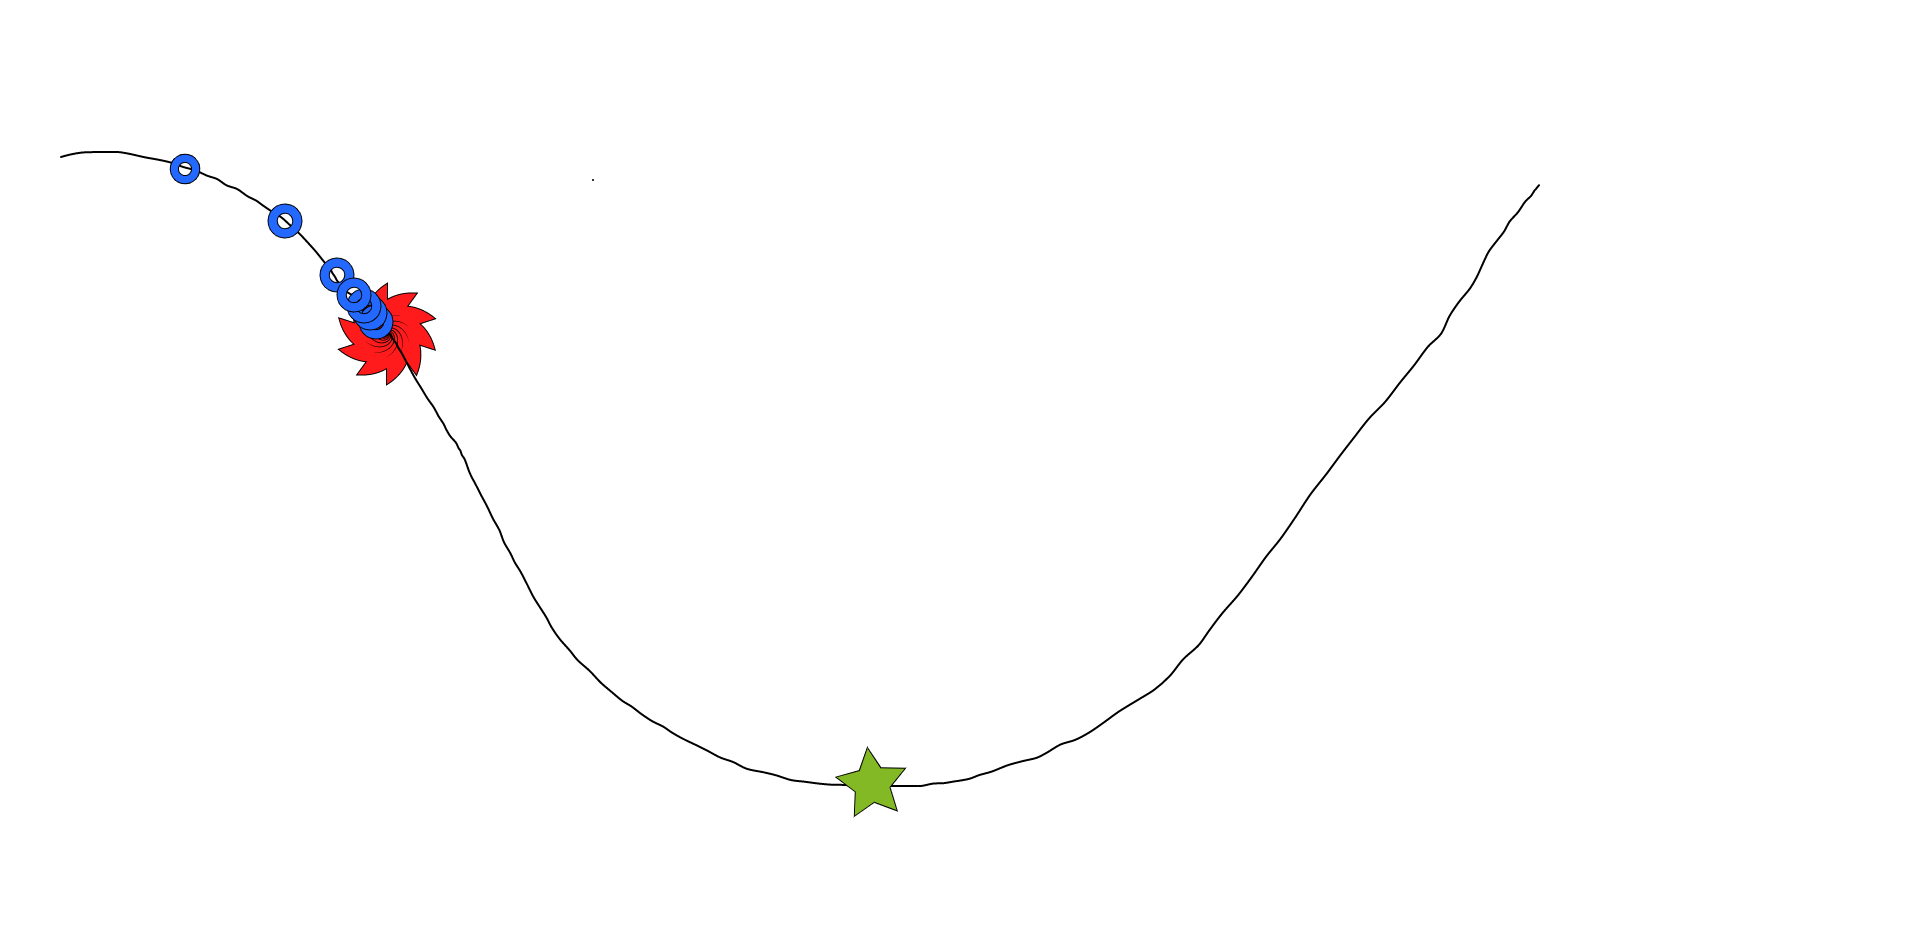
\includegraphics[width=120px]{images/sufficient_reduction.png}
		\end{center}
	\end{itemize}
\end{frame}


\begin{frame}{Algorithm Assumptions}
	\begin{itemize}
		\item The algorithm can satisfy the efficiency condition if it produces trial points that reduce the objective's model:
		\begin{align*}
			& m_f^{(k)}\left(\xk\right) - m_f^{(k)}\left(x^{(k+1)}\right) \\
			& \ge c_1 \chi^{(k)} \min \left\{
				\frac{\chi^{(k)}}{1 + \left\|\nabla^2 m_f^{(k)}\left(x^{(k)}\right)\right\|},
				\Delta_k, 1\right\}
		\end{align*}
		\item The accuracy condition ensures:
		\begin{align*}
			\left\|\nabla m_f^{(k)}\left(x^{(k)}\right) - \nabla f\left(x^{(k)}\right)\right\| \le c_2 \Delta_k
		\end{align*}
	\end{itemize}
\end{frame}


\begin{frame}{The Algorithm for Linear Constraints}
	\begin{itemize}
		\item The linear algorithm is an implementation of the algorithm within \cite{CONEJO2013324}
		\item We satisfy the hypothesis presented in this article
		\item We need sample points to ensure the model satisfies the accuracy condition
\begin{align*}
		\left\|\nabla m_f^{(k)}\left(x^{(k)}\right) - \nabla f \left(x^{(k)}\right)\right\| \le c_2 \Delta_k
\end{align*}
		\item We were able to rely on classic model improving algorithms by choosing an ellipsoidal sample region
% 		\item Constructing a feasible ellipsoid also sets the foundation for the non-linear sample region
	\end{itemize}
\end{frame}


\begin{frame}{Feasible Derivative Free Trust Regions}
	\begin{itemize}
		\item The outer trust region:
			\begin{itemize}
				\item Is an $L_{\infty}$ ball
				\item Can contain infeasible points
				\item Contains both the other trust regions.
			\end{itemize}
		\item The sample region:
			\begin{itemize}
				\item Used to construct sample points
				\item Must become feasible
				\item Must be constructed from the previous models
% 				\item Has an ellipsoidal shape
			\end{itemize}
		\item The search region:
			\begin{itemize}
				\item Used to construct trial points
				\item Must become feasible
				\item Must allow for sufficient reduction
			\end{itemize}
	\end{itemize}
\end{frame}


\begin{frame}{Sample Region Requirements}
	\begin{itemize}
		\setlength\itemsep{1.5em}
		\item The sample region is given by
\begin{align*}
\left\{x \in \Rn \bigg | \left(x - c^{(k)}\right)^TQ^{(k)}\left(x - c^{(k)}\right) \le \frac 1 2 \delta_k^2 \right\}
\end{align*}
		\item The condition number of $Q^{(k)}$ must be bounded
		\item The ellipsoid must be near the current iterate
		\item The ellipsoid must be feasible
	\end{itemize}
\end{frame}


\begin{frame}{Example Trust Region}
	\begin{center}
% 	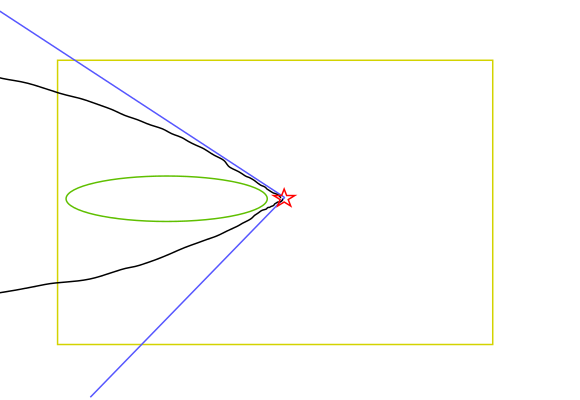
\includegraphics[width=300px]{images/trust_regions.png}
		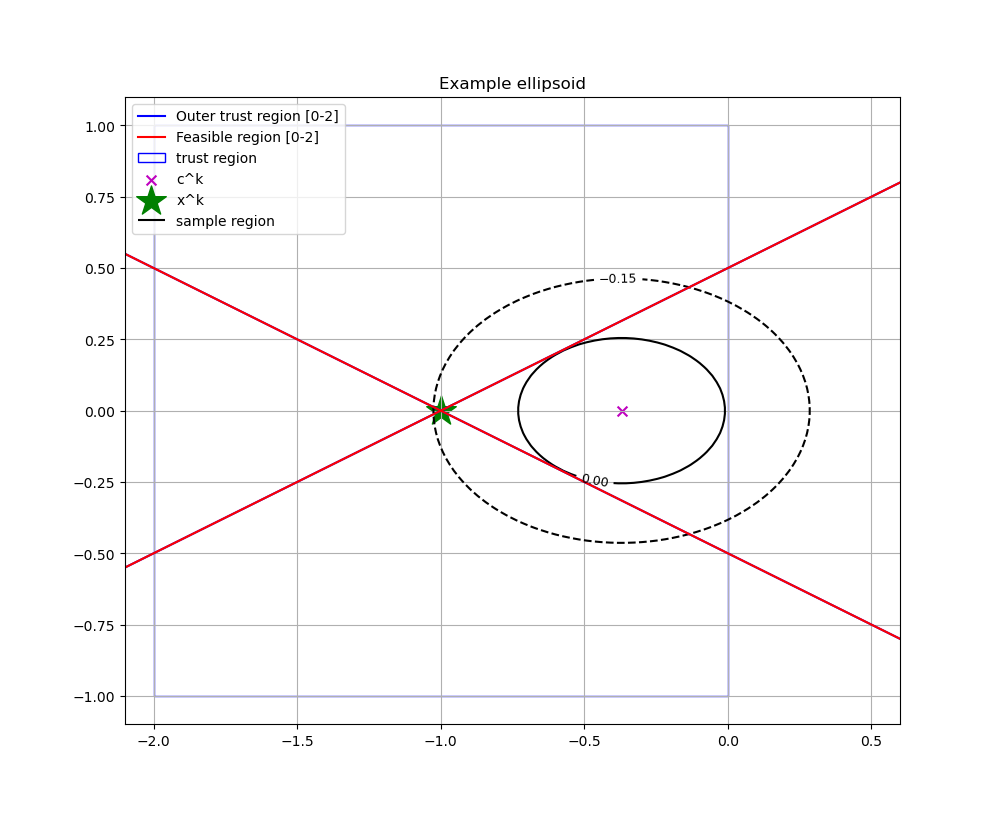
\includegraphics[width=200px]{images/example_ellipsoid.png}
	\end{center}
% \includegraphics[width=300px]{images/ellipse_at_current_iterate.png}
\end{frame}


\begin{frame}{Ellipsoid Construction}
	\begin{itemize}
		\item Construct direction feasible with respect to nearly active constraints
		\begin{center}
			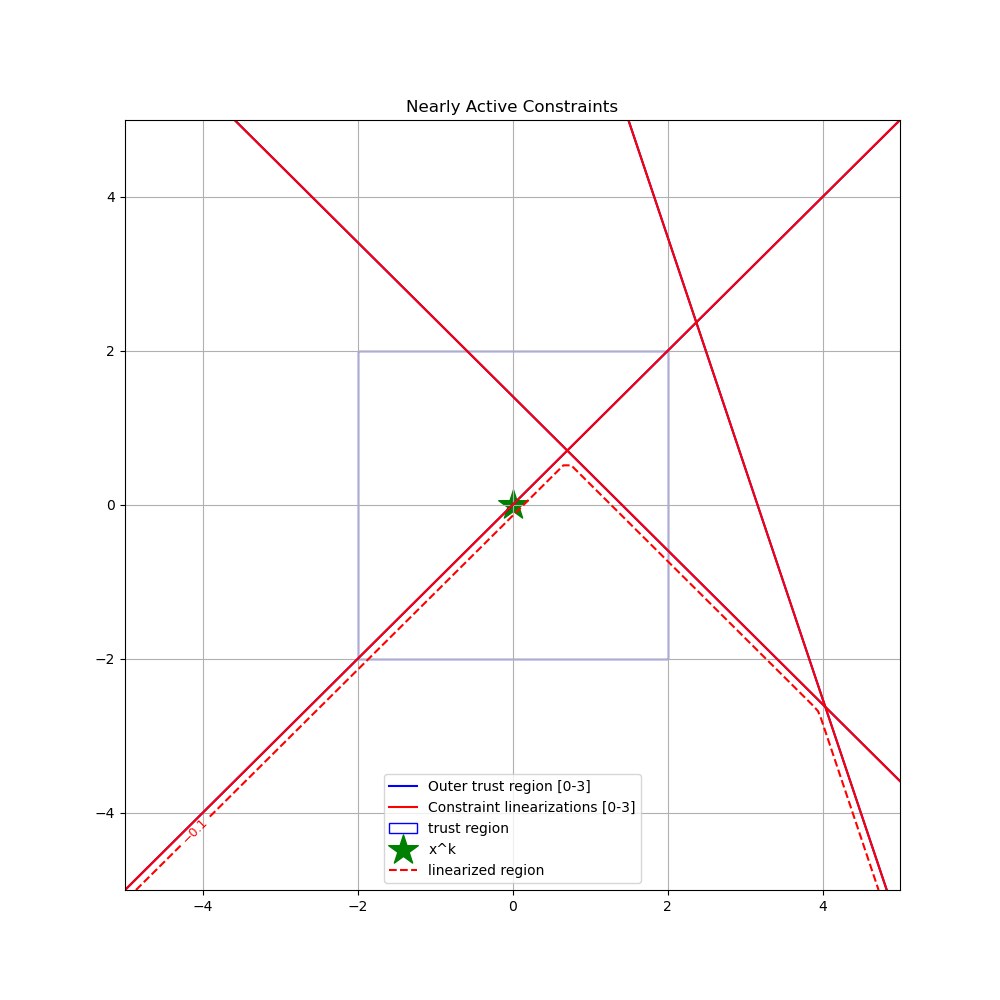
\includegraphics[width=150px]{images/active_constraints.png}
		\end{center}
	\end{itemize}
\end{frame}

\begin{frame}{Ellipsoid Construction}
	\begin{itemize}
		\item Construct direction feasible with respect to nearly active constraints
		\item Find the widest open rate of a second order cone
		\begin{center}
% 			Include 3d picture
%			Nearly active constraints
			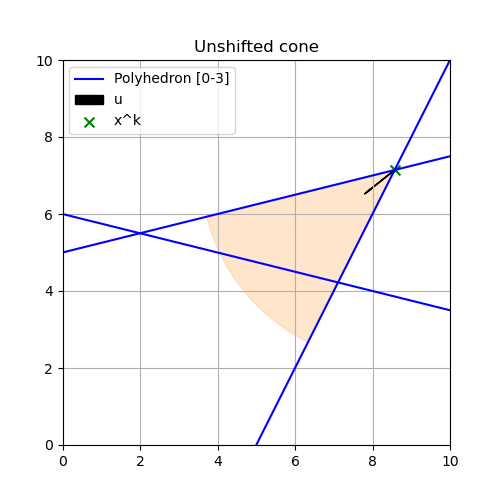
\includegraphics[width=100px]{images/unshifted_cone.png}
			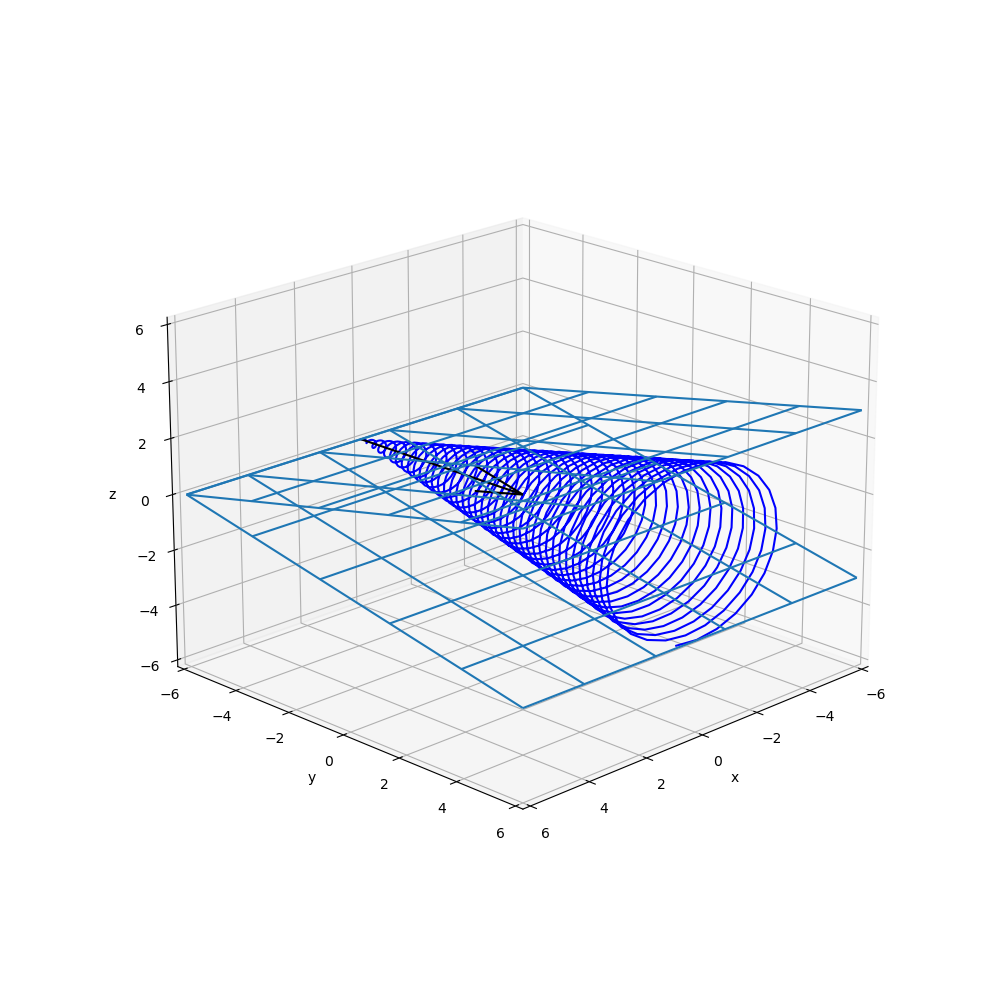
\includegraphics[width=100px]{images/second_order_cone.png}
		\end{center}
		\item Compute an ellipsoid within this cone
	\end{itemize}
\end{frame}


\begin{frame}{Linear Algorithm Summary}
	\begin{itemize}
		\item We implemented accurate model construction by constructing a feasible ellipsoid
		\item We set the search region to the intersection of the trust region and the 
		\item By satisfying the conditions for Conejo, we know the criticality measure goes to zero
	\end{itemize}
\end{frame}

% \begin{frame}{Ellipsoid Construction}
% 	
% 	<Image of ellipsoid in a cone>
% \end{frame}

% 
% \begin{frame}{Feasible Derivative Free Algorithm Part 2}
%	 \begin{itemize}
%		 \item 
%		 \item This can be satisfied using the Generalized Cauchy Point
%		 \item The accuracy condition requires: 
%		 \item To satisfy this, we require the ellipsoid we find to have bounded condition number
%	 \end{itemize}
% \end{frame}


\begin{frame}{Nonlinear Algorithm}
	To handle inaccurate constraint models, 
	we chose to buffer the sample and search regions from the constraint boundaries
	
	\begin{center}
		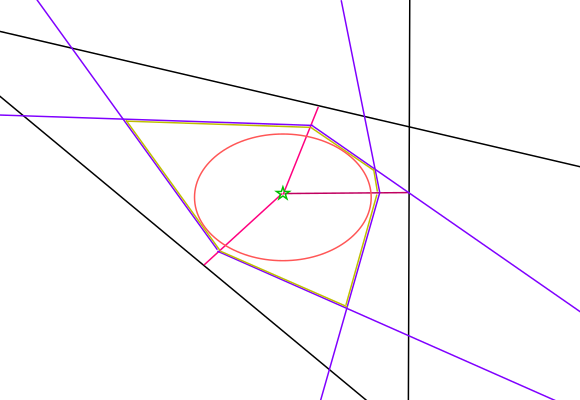
\includegraphics[width=200px]{images/completed_2.png}
	\end{center}
	
% 	\begin{block}{Buffered Region Challenges:}
% 		\begin{itemize}
% 			\item Show sufficient reduction within this buffered region
% 			\item Show that the criticality measure approximates the real criticality measure
% 			\item Handle 
% 		\item Recover a feasible ellipsoid when required
% 		\end{itemize}
% 	\end{block}
\end{frame}

\begin{frame}{Buffering Cones}
	We construct the buffering cones as follows:
	\begin{center}
		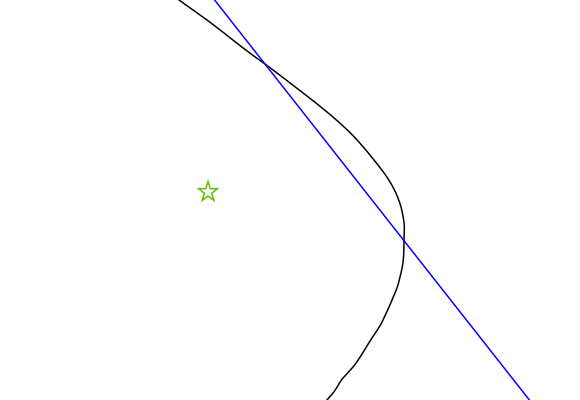
\includegraphics[width=200px]{images/explanation_1.png}
	\end{center}
\end{frame}


\begin{frame}{Buffering Cones}
	The cone's vertex is the linearizations zero, scaled towards the current iterate
	\begin{center}
		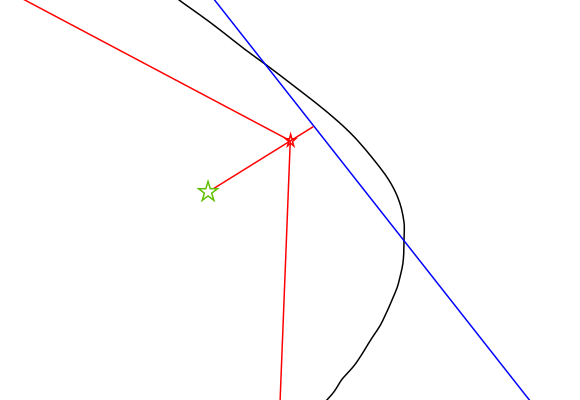
\includegraphics[width=200px]{images/explanation_2.png}
	\end{center}
\end{frame}


\begin{frame}{Buffering Cones}
	As the $\dk \to 0$, the buffered region approaches the linearization.
	\begin{center}
		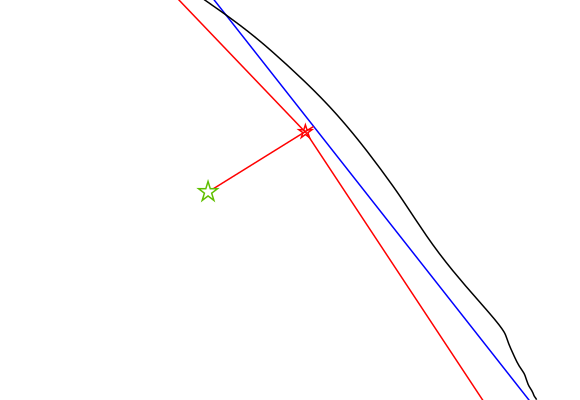
\includegraphics[width=200px]{images/explanation_3.png}
	\end{center}
\end{frame}


\begin{frame}{Buffering Cones}
	We show the intersection of these cones is feasible for small $\Delta_k$
 	\begin{center}
 		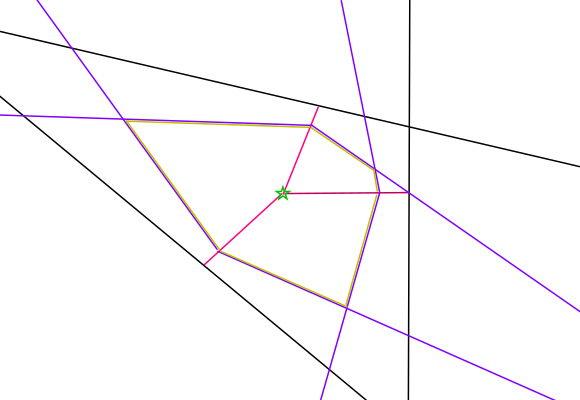
\includegraphics[width=125px]{images/completed_1.png}
 	\end{center}
\end{frame}

\begin{frame}{Buffering Cones}
	\begin{block}{Theorem 4.24}
		Suppose that $C^{(i, k)}$ is the $i$-th's constraints buffering cone during iteration $k$,
		that $F$ is the true feasible region,
		and that $\mathcal A^{(k)}$ is the set of active constraints at iteration $k$. \\
		There exists a $\Delta_{\textrm{feasible}} > 0$ such that
		if $\Delta_k \le \Delta_{\textrm{feasible}}$, then 
		$\left[\cap_{i \in \mathcal A^{(k)}} C^{(i, k)} \right] \cap \left[B_{\infty}\left(\xk, \Delta_{k}\right) \cup B_{\infty}\left(\xk, \Delta_{k+1}\right)\right] \subseteq F$.
	\end{block}
\end{frame}

\begin{frame}{Conservative Construction}
	We can reuse the sample region construction for linear constraints
	\begin{center}
		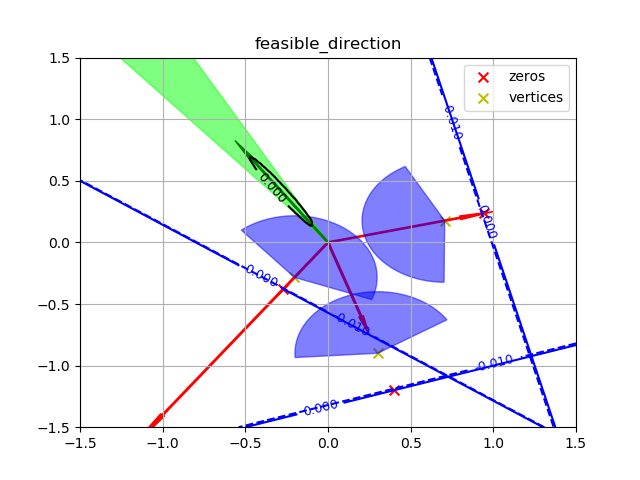
\includegraphics[width=200px]{images/feasible_direction.png}
	\end{center}
\end{frame}



% \begin{frame}{Buffering Cones, Delete this}
% 	\begin{itemize}
% 		\item Also, the paper does not provide a mechanism for satisfying the accuracy condition
% 		\[\|\nabla m_f(x) - \nabla f(x)\| \le \epsilon_g \dk \]
% 		\item This usually not an issue, as any point can be added to the sample set to
% 		replace ill-poised points
% 		\begin{center}
% 			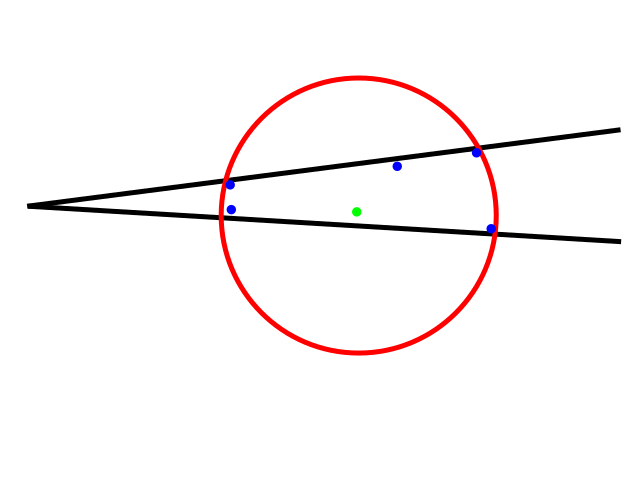
\includegraphics[width=120px]{images/impossible_poised.png}
% 		\end{center}
% 		\item We had to show that we can still find a ``large" enough region to choose sample points
% 	\end{itemize}
% \end{frame}


\begin{frame}{No Buffered Reduction Possible}
	While $\Delta_k$ is large, the buffered region may not provide reduction
% 	Because $\Delta_k$ must be sufficiently small, we must perform an explicit efficiency check within the algorithm
	\begin{center}
		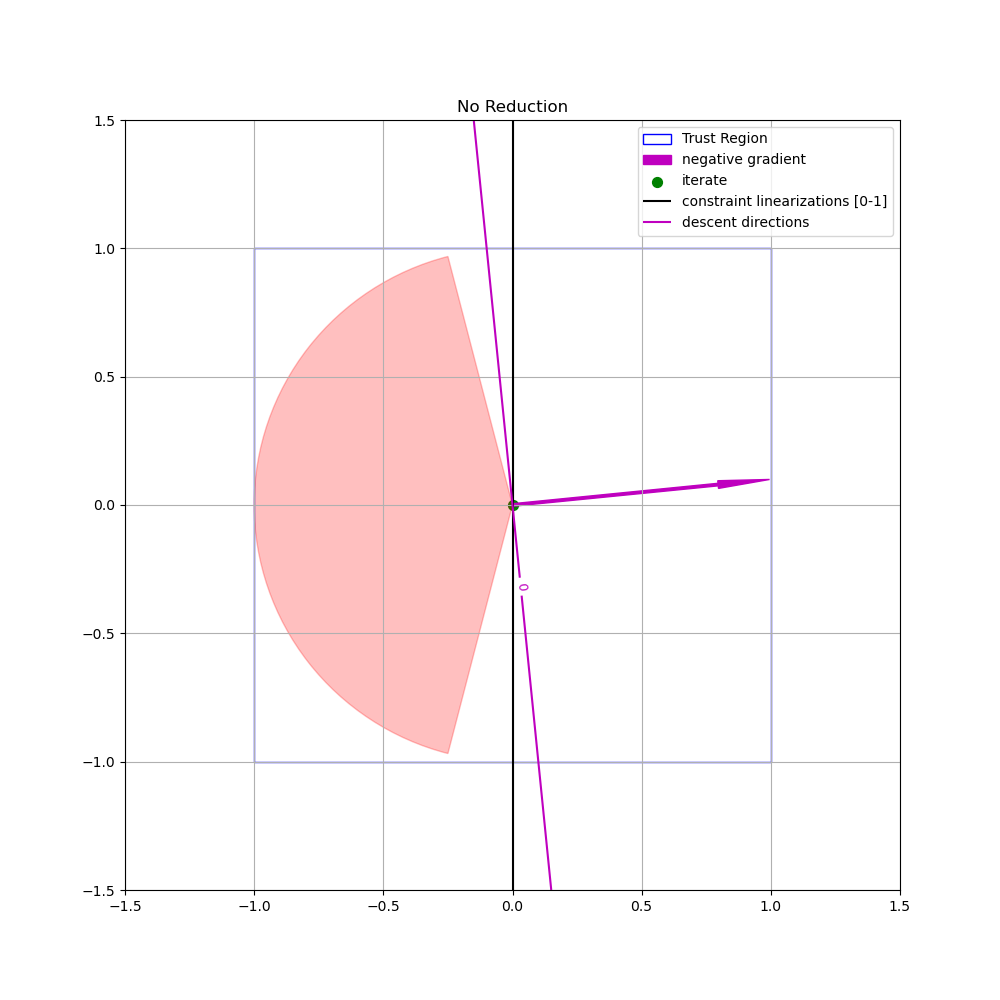
\includegraphics[width=175px]{images/no_reduction.png}
	\end{center}
% 		\item Thus, we constructed a point that satisfies the efficiency condition within the smaller region
% 		\item Only works for small $\Delta_k$.
\end{frame}


\begin{frame}{Sufficient Reduction}
	\begin{itemize}
		\item By buffering the trust region, we limit trial points
		\item We can no longer use well-known algorithms for computing an efficient trial
		\begin{block}{Theorem 4.27}
			If $\chi^{(k)} \ge \kappa_{\chi} \Delta_k^{p_{\Delta}}$ and $\Delta_k \le \Delta_{\textrm{sf}}$,
			then there is a $v$ in the buffered region that satisfies the efficiency condition.
		\end{block}
		\item Requires small $\Delta_k$, so we must explicitly check for reduction.
		
	\end{itemize}
% Could talk about the details here
\end{frame}


\begin{frame}{Feasible Trial Point}
	Moving a solution to the buffered region
	\begin{center}
		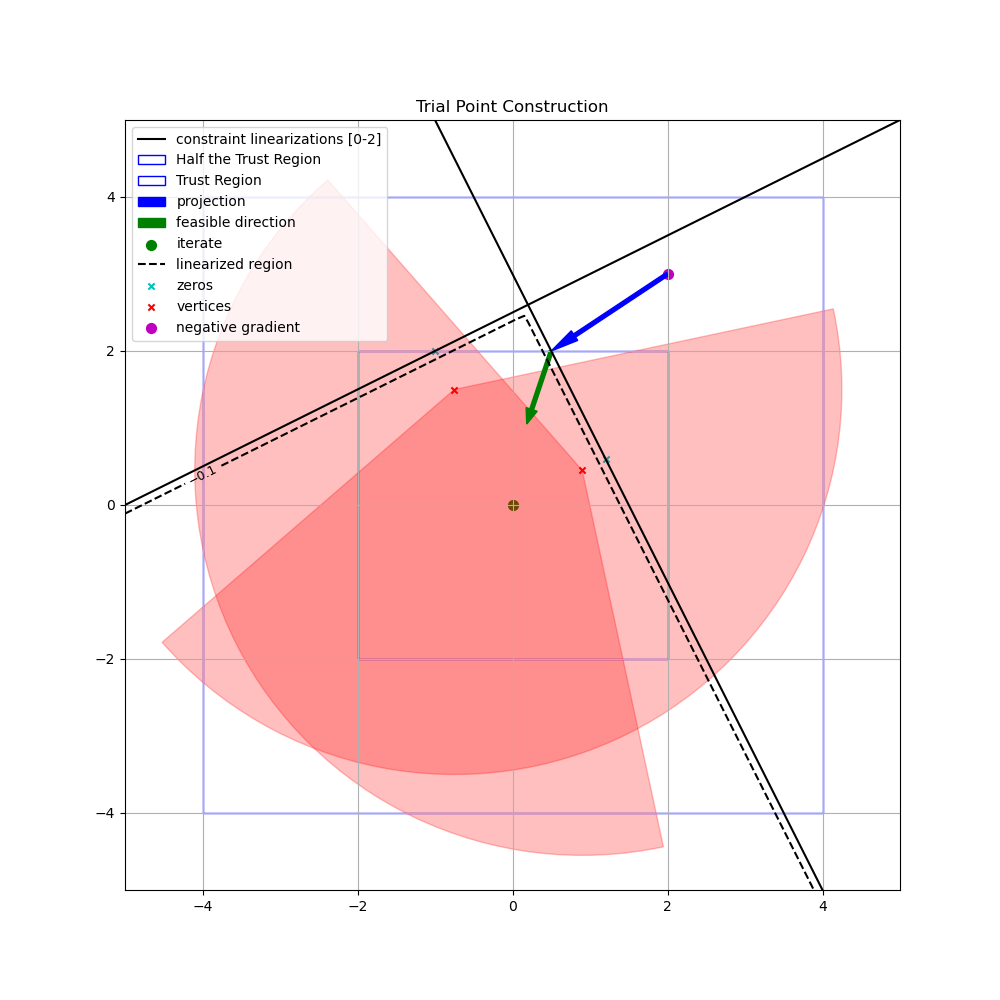
\includegraphics[width=175px]{images/trial_point_constructions.png}
	\end{center}
\end{frame}


\begin{frame}{Criticality Measure}
	\begin{itemize}
		\item The classic criticality for convex constraints is
\begin{align*}
\chi(x) = \left\|\xk - \proj_{\feasible}\left(x - \nabla f(x)\right)\right\|
\end{align*}
		\item We only have access to models:
\begin{align*}
\chi_m^{(k)}(x) = \left\|\xk - \proj_{\feasiblek}\left(x - \nabla m_f^{(k)}(x)\right)\right\|
\end{align*}
% 		\item This is still sufficient for general constraints
		\item We showed that both $\left|\chi_m^{(k)}\left(\xk\right) - \chi\left(\xk\right)\right| \to 0$ 
% 		and $\left|\chi_m^{(k)}\left(\xk\right) - \chi_m^{(l)}\left(x^{(l)}\right)\right| \to 0$
	\end{itemize}
\end{frame}



\begin{frame}{Uniform Convergence of Criticality Measure}
	The criticality measure changes with constraint model changes
	\begin{center}
		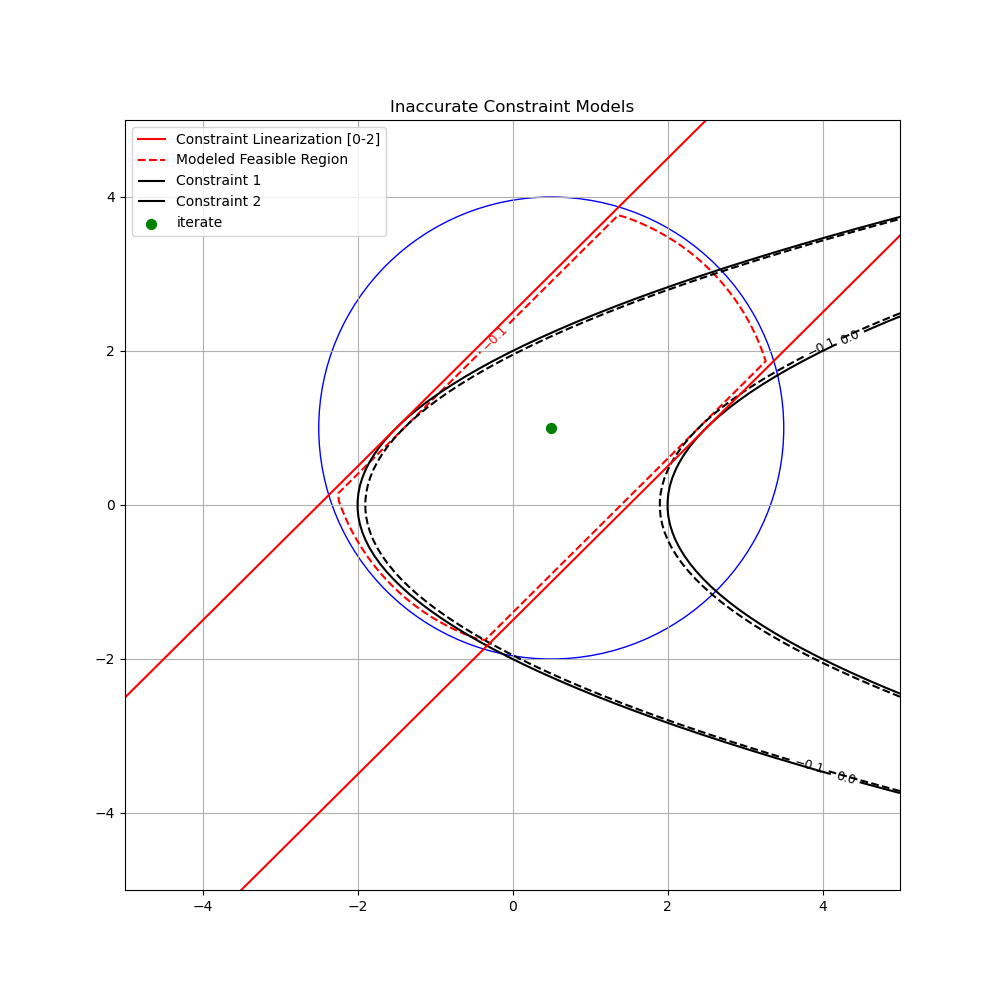
\includegraphics[width=150px]{images/modeled_constraints_2.png}
		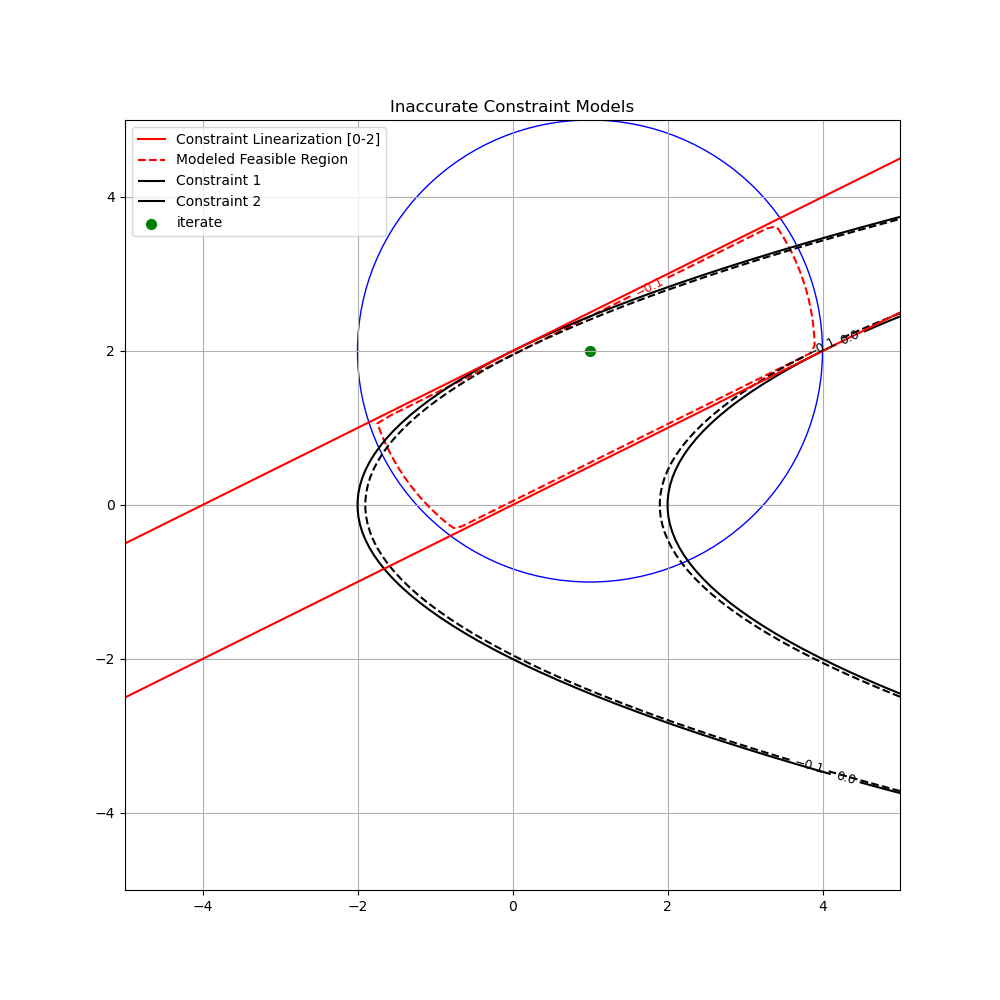
\includegraphics[width=150px]{images/modeled_constraints_3.png}
	\end{center}
\end{frame}


% \begin{frame}{Criticality Measure, Delete this}
% \color{red}
% 	\begin{itemize}
% 		\item The algorithm's criticality measure used the projection operator onto the true constraints
% 		\item We only use the projection onto the linearization of the model constraints
% 	\end{itemize}
% 	\begin{center}
% 		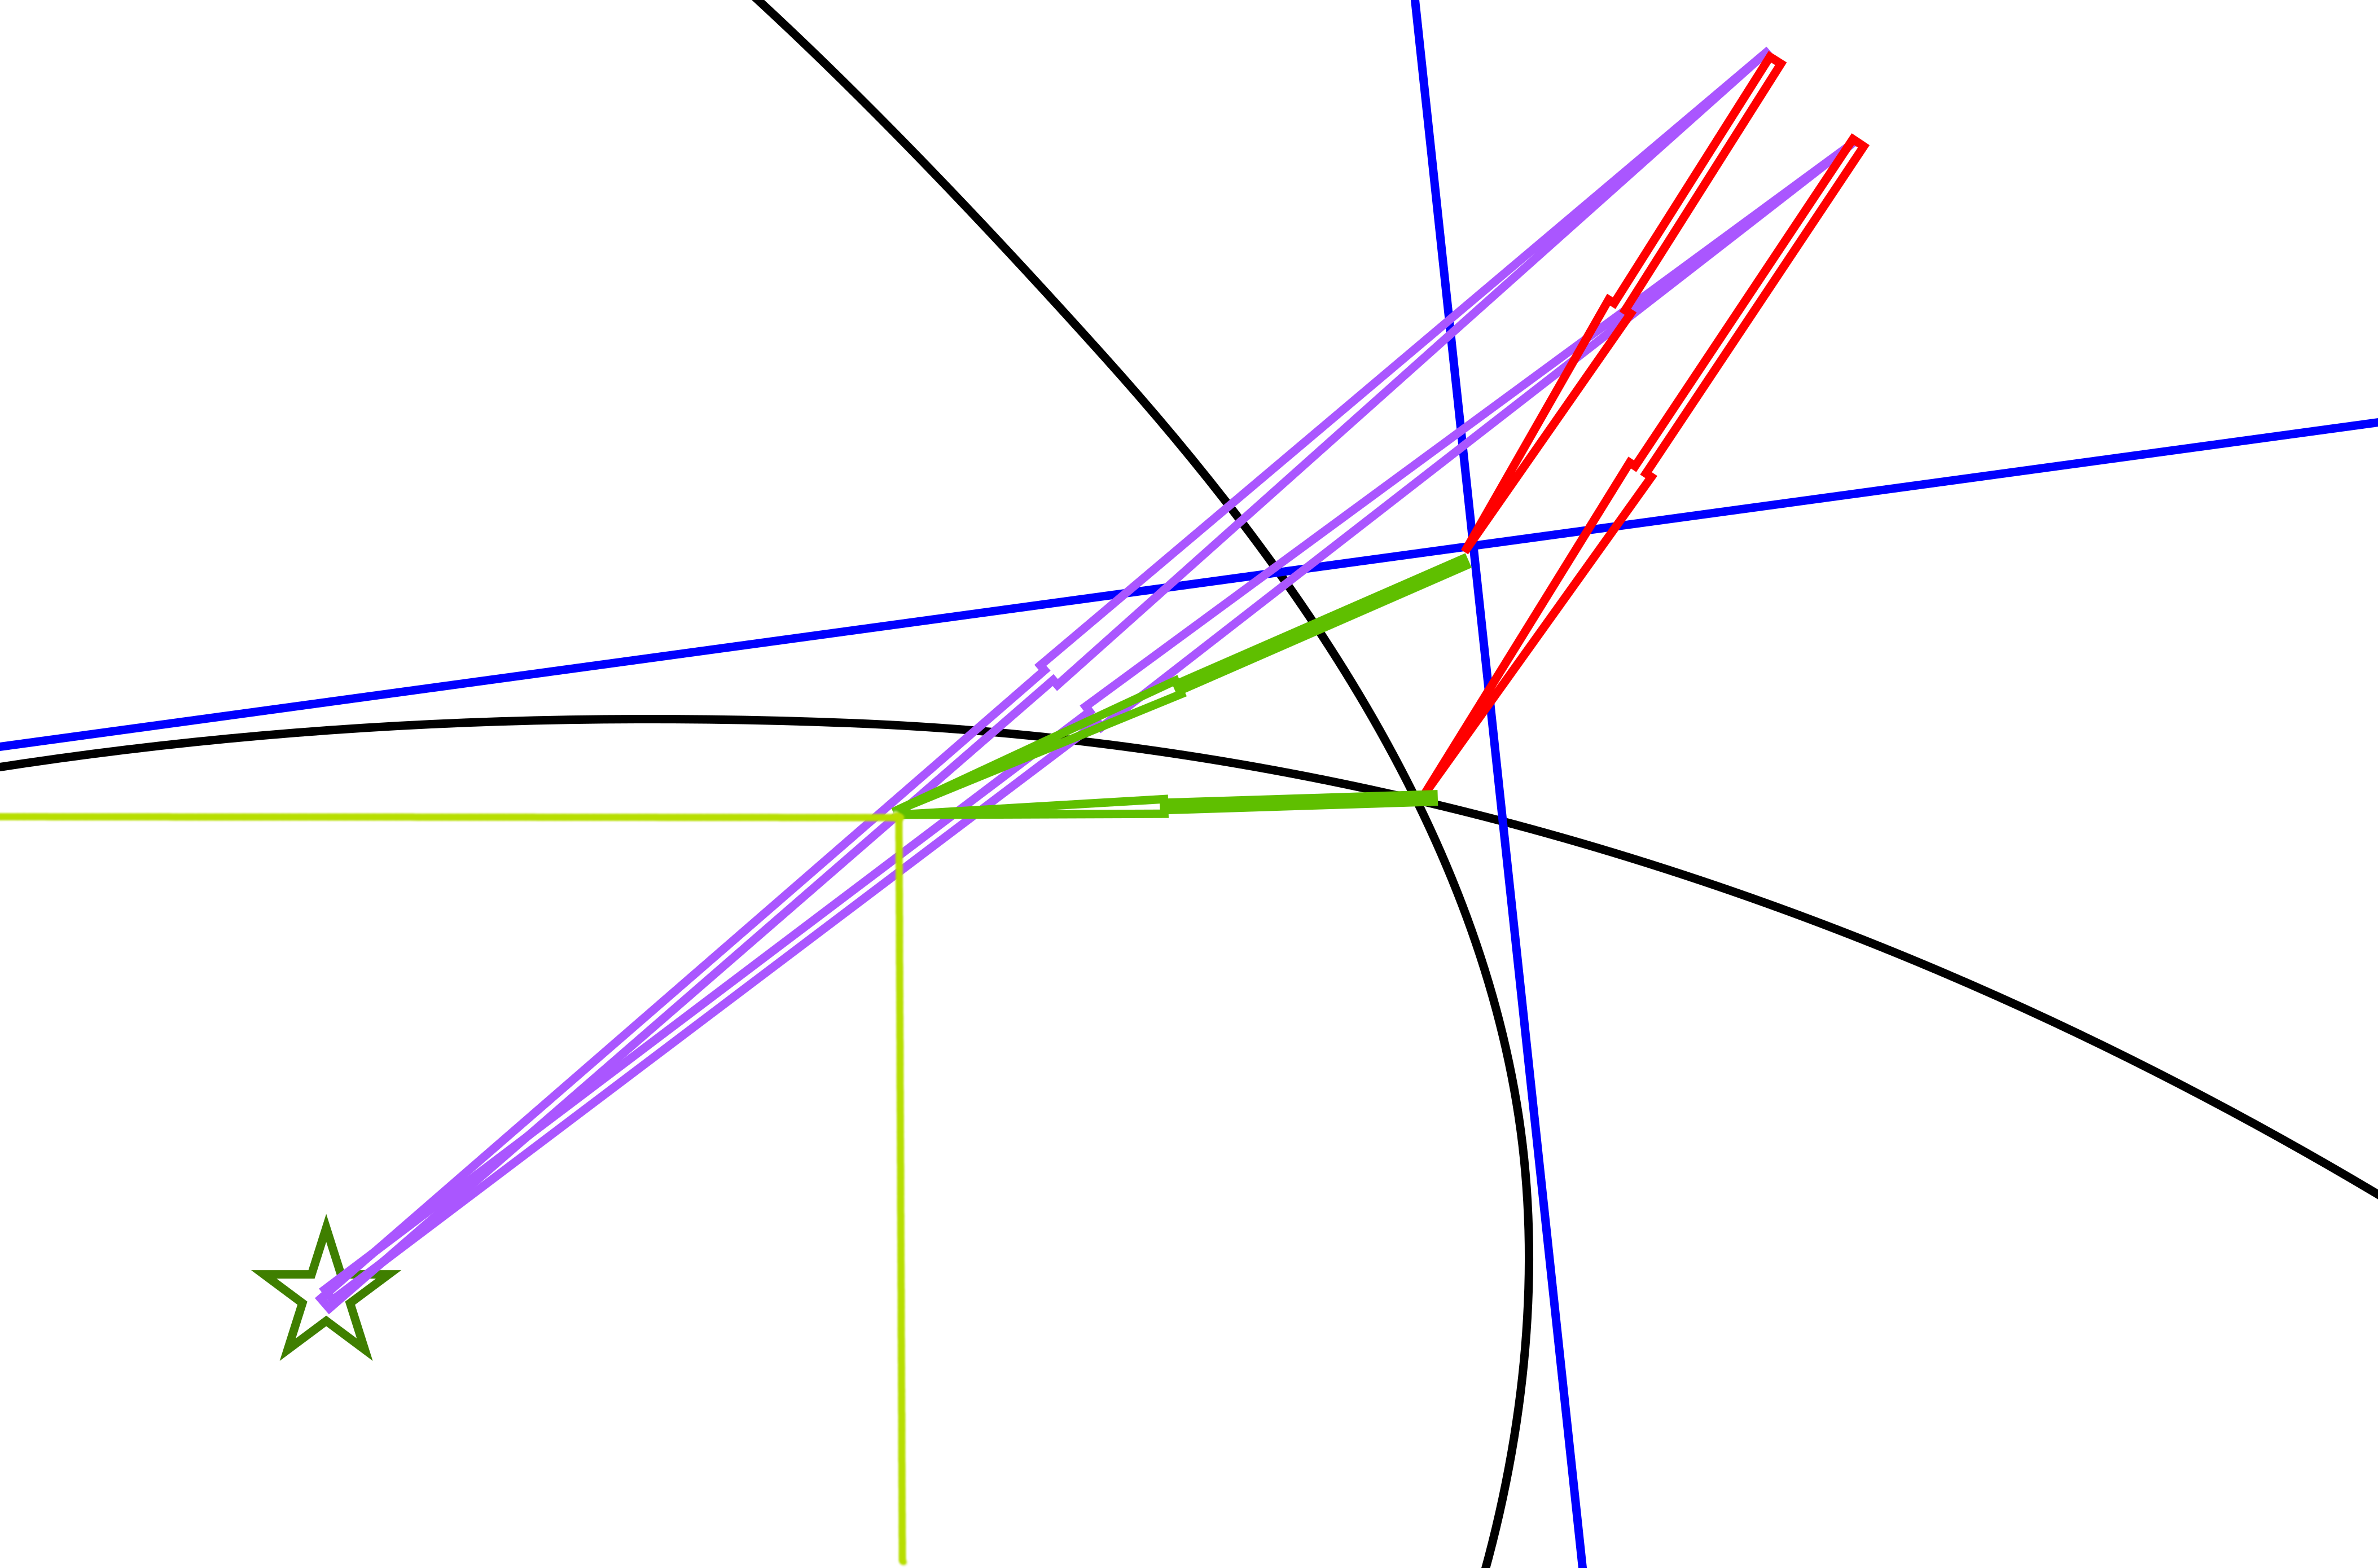
\includegraphics[width=150px]{images/criticality_measure.png}
% 	\end{center}
% \color{black}
% \end{frame}


\begin{frame}{Bounded Projection}
	Projections don't move far when some constraints are perturbed...
	\begin{center}
		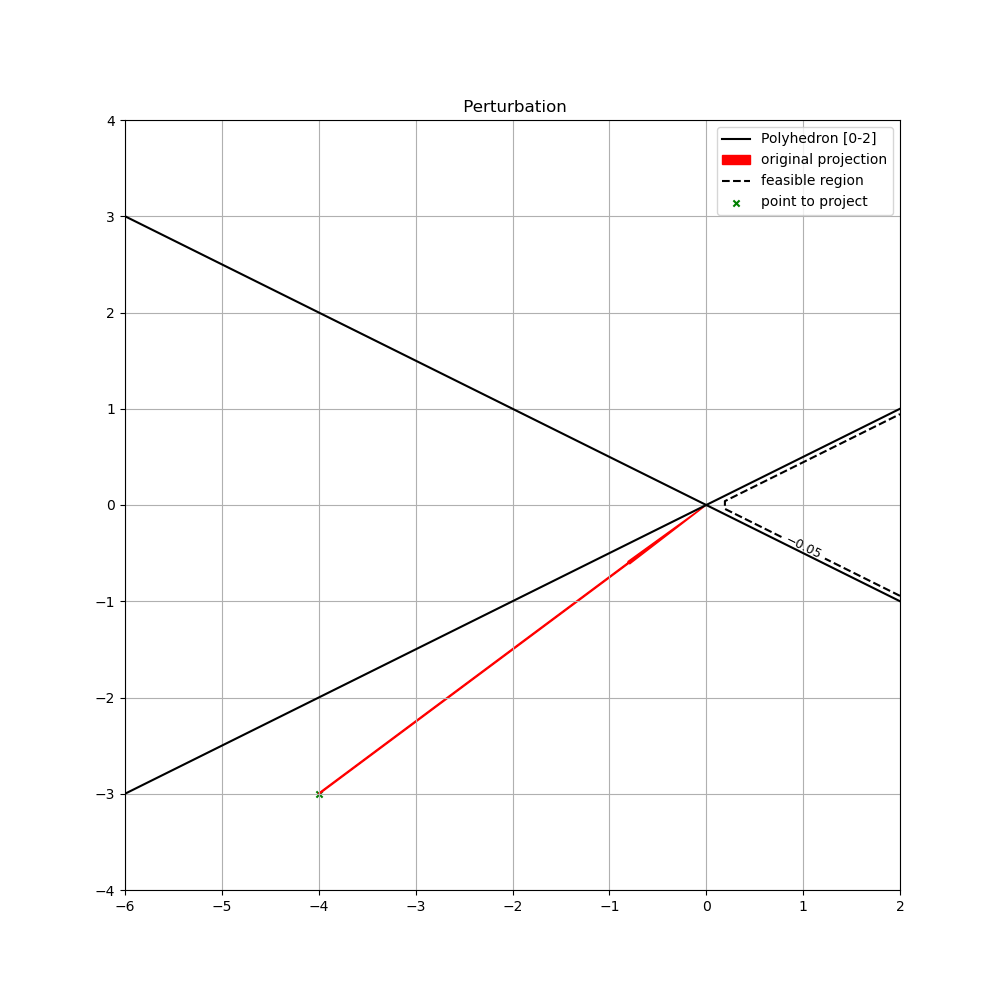
\includegraphics[width=150px]{images/hoffman_0.png}
		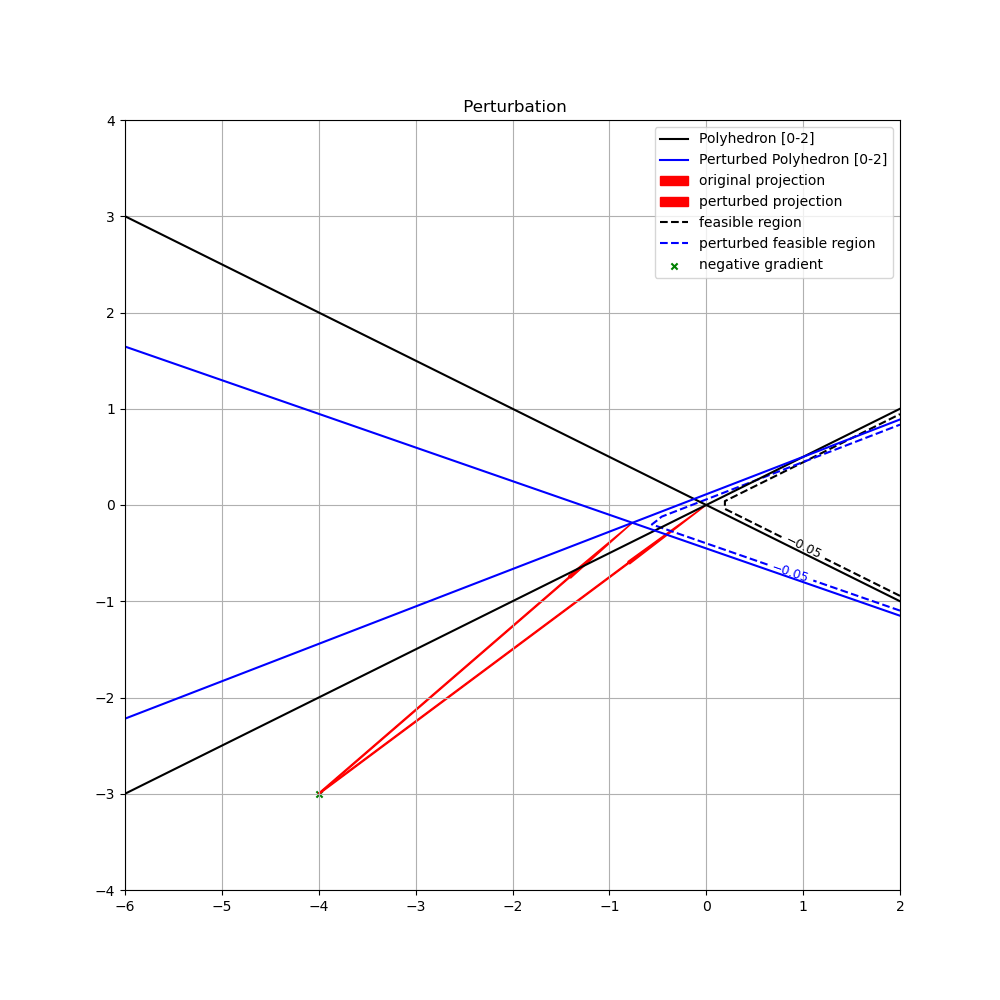
\includegraphics[width=150px]{images/hoffman_1.png}
	\end{center}
\end{frame}


\begin{frame}{Bounded Projection}
	...but projections can for narrow constraints
	\begin{center}
		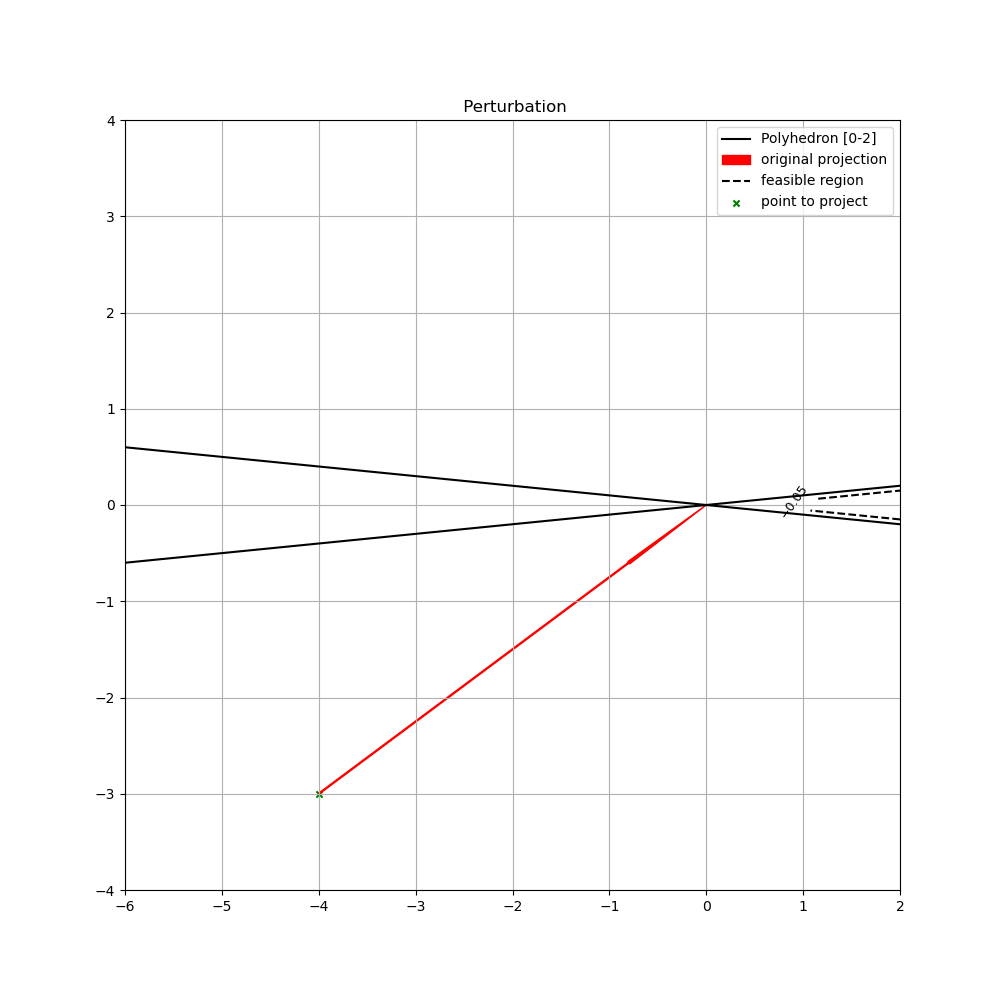
\includegraphics[width=150px]{images/hoffman_2.png}
		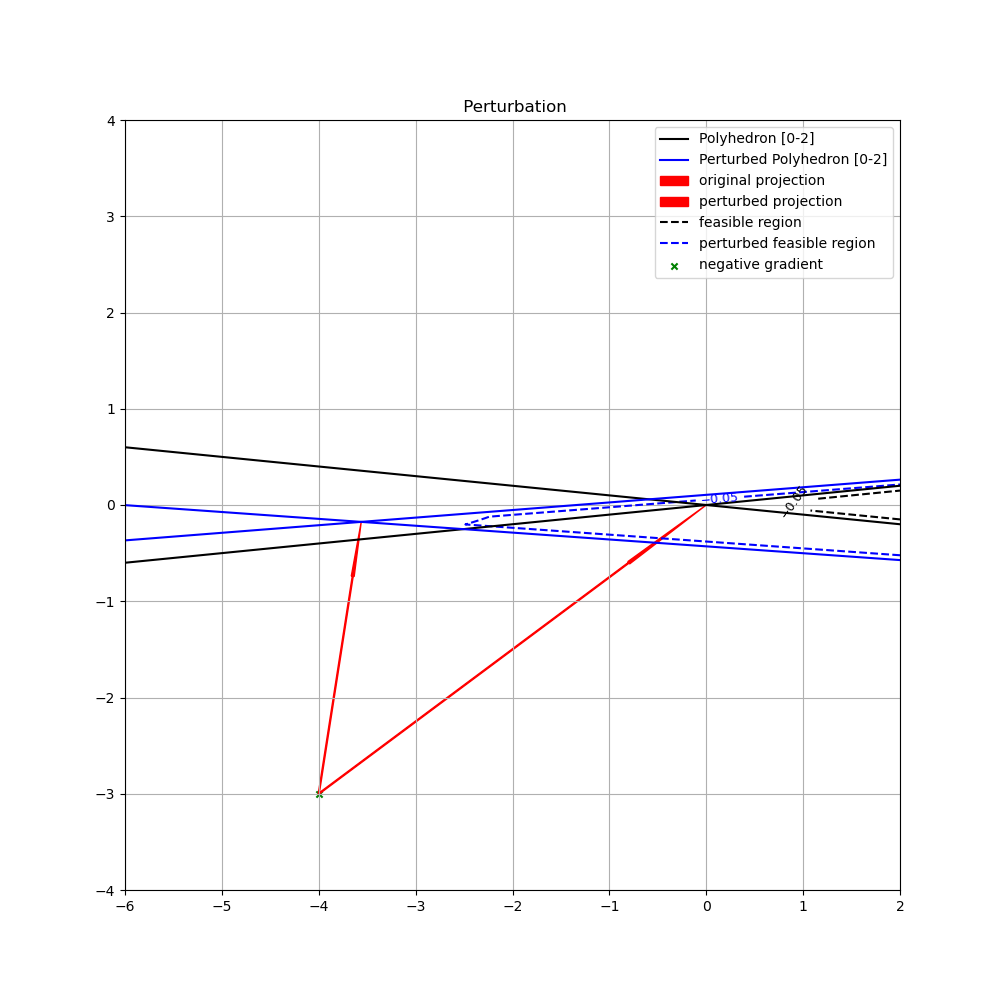
\includegraphics[width=150px]{images/hoffman_3.png}
	\end{center}
\end{frame}



\begin{frame}{Bounded Projection}
	Only constraints near the current iterate can make a small angle
	\begin{center}
		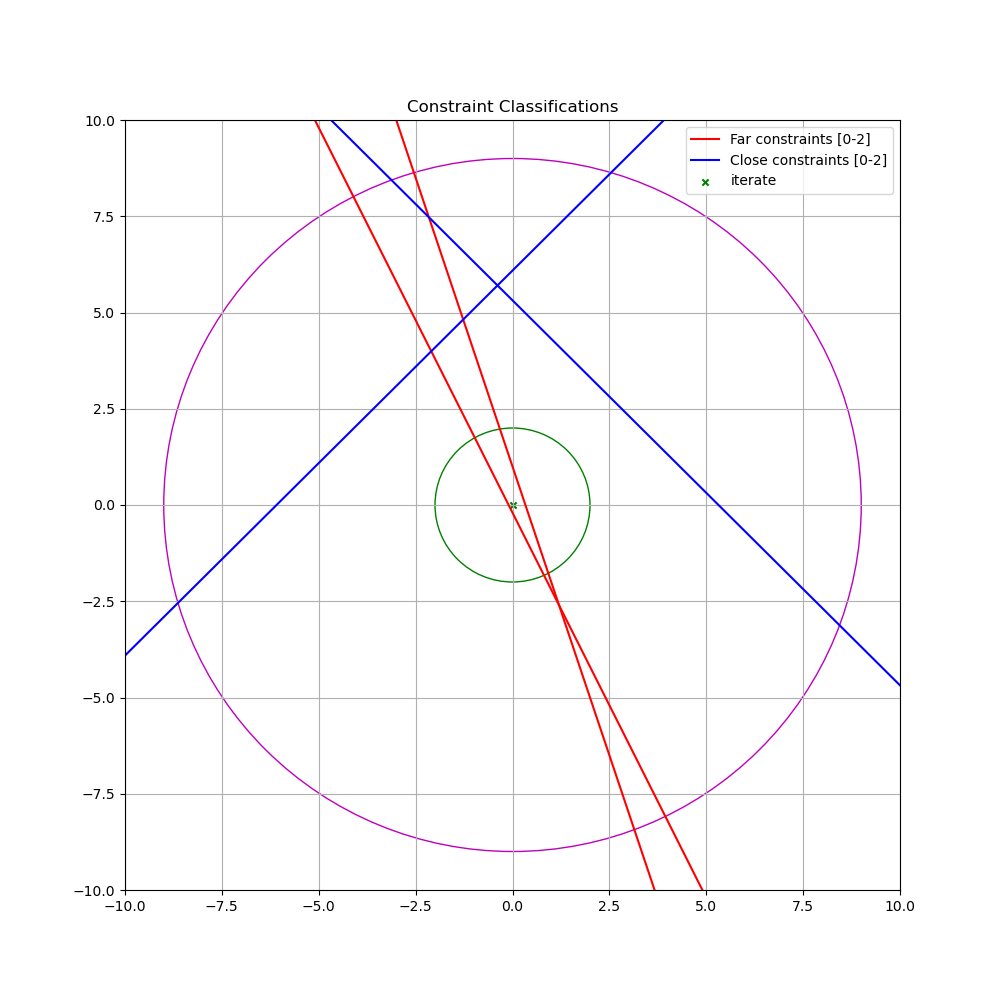
\includegraphics[width=175px]{images/classification.png}
	\end{center}
\end{frame}


\begin{frame}{Bounded Projection}
	\begin{itemize}
		\item How far a projection onto the linearized feasible region moves depends on
		$
			\min_{\|u\| = 1, u \ge 0} \left\|\sum_{i} u_i \nabla \hat c_i\left(\xk\right)\right\|
		$
		\item This quantity is bounded by a regularity assumption
		\begin{block}{Theorem 4.41}
			Let $F_m^{(k)}$ and $F_c^{(k)}$ be the model's and constraints linearized feasible region for iteration $k$ respectively,
			and $\neggrad = \xk - \nabla m_f\left(\xk\right)$. Then,
			\begin{align*}
				\begin{array}{ccc}
					\left\|P_{F_m^{(k)}}\left(\neggrad\right)
					-  P_{F_m^{(l)}}\left(\neggrad\right)\right\| & \to 0 & \quad \textrm{and} \\
					\left\|P_{F_m^{(k)}}\left(\neggrad\right)
					-  P_{F_c^{(k)}}\left(\neggrad\right)\right\| & \to 0. &
				\end{array}
			\end{align*}
		\end{block}
	\end{itemize}
\end{frame}



\begin{frame}{Regularity Assumption}
\begin{itemize}
\item The Mangasarian-Fromovitz constraint qualification requires
\begin{align*}
\forall x^{\star}, \exists d \in \Rn, \forall i, \\
c_i\left(x^{\star}\right)=0 \wedge \chi\left(x^{\star}\right) = 0 \Longrightarrow \nabla c_i\left(x^{\star}\right)^T d < 0 
\end{align*}
\item We strengthened this qualification:
\begin{align*}
\forall x \exists d \in \Rn\; \forall i, \nabla c_i\left(x\right)^T d < 0
\end{align*}
\end{itemize}
\end{frame}


\begin{frame}{Regularity Assumption}
	Only assume regularity for nearly active constraints
	\begin{center}
		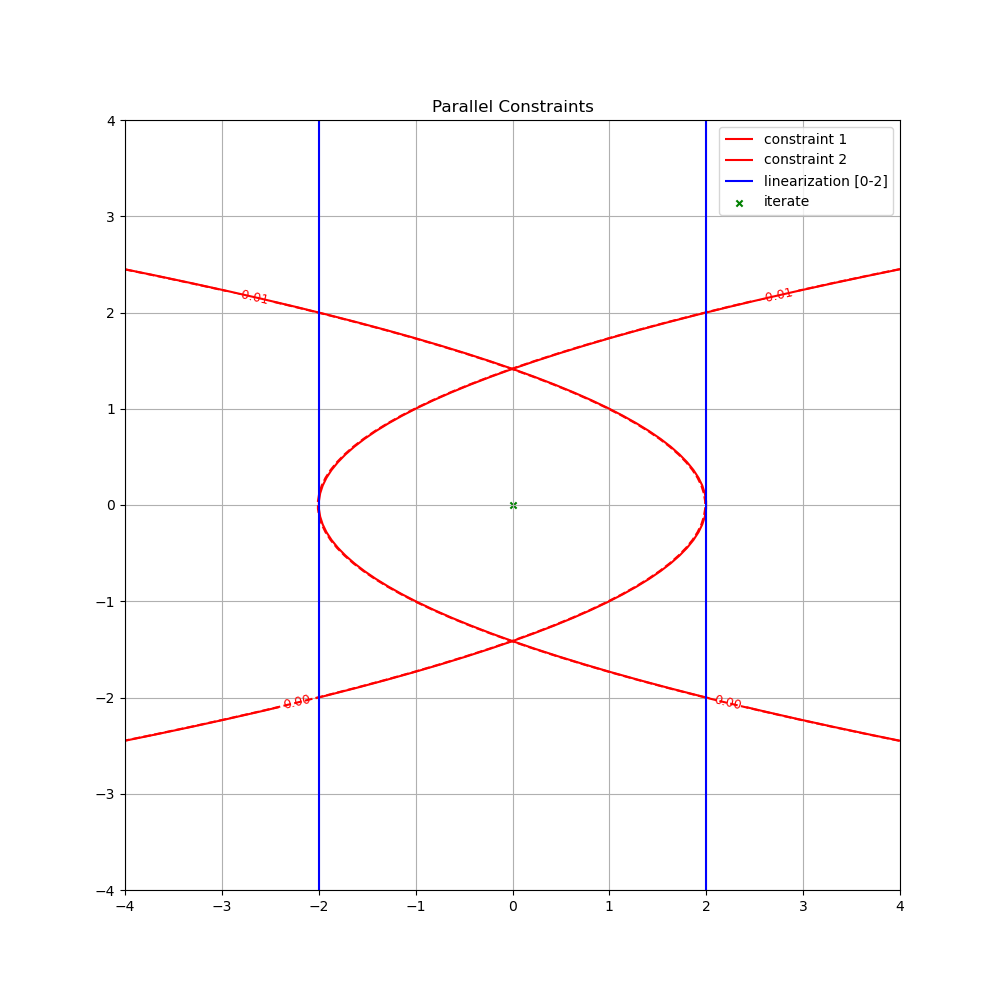
\includegraphics[width=175px]{images/local_regularity.png}
	\end{center}
\end{frame}

\begin{frame}{Regularity Assumption}
\begin{itemize}
\item The Mangasarian-Fromovitz constraint qualification requires that for any critical point 
\begin{align*}
\forall x^{\star}, \exists d \in \Rn, \forall i, \\
c_i\left(x^{\star}\right)=0 \wedge \chi\left(x^{\star}\right) = 0 \Longrightarrow \nabla c_i\left(x^{\star}\right)^T d < 0 
\end{align*}
\item We strengthened this qualification:
\begin{align*}
\xout{\forall x \exists d \in \Rn\; \forall i, \nabla c_i\left(x\right)^T d < 0} \\
\forall x \exists d \in \Rn\; \forall i, \nabla c_i\left(x\right) \approx 0 \Longrightarrow \nabla c_i\left(x\right)^T d < 0 \\
\end{align*}
\end{itemize}
\end{frame}

\begin{frame}{Regularity Assumption}
	We ensure a uniform bound on the ``width" of the feasible set's tangent cone
	\begin{center}
% 		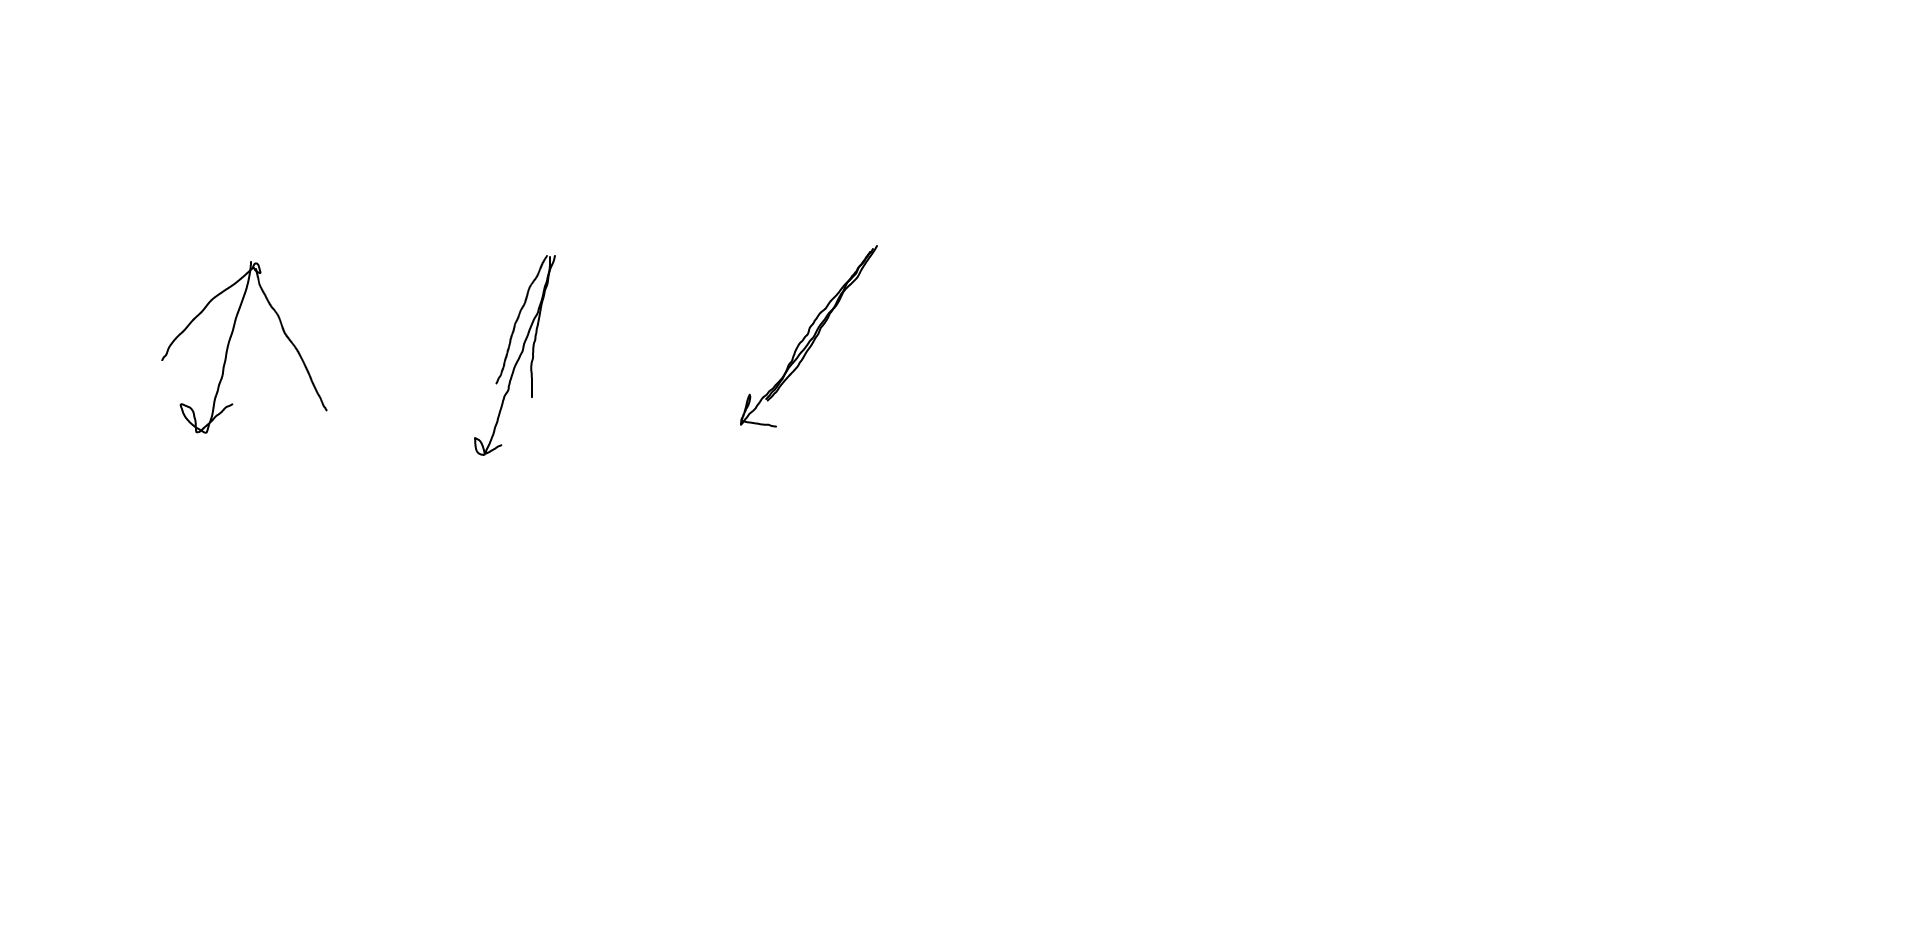
\includegraphics[width=200px]{images/uniform_regularity.png}
% 		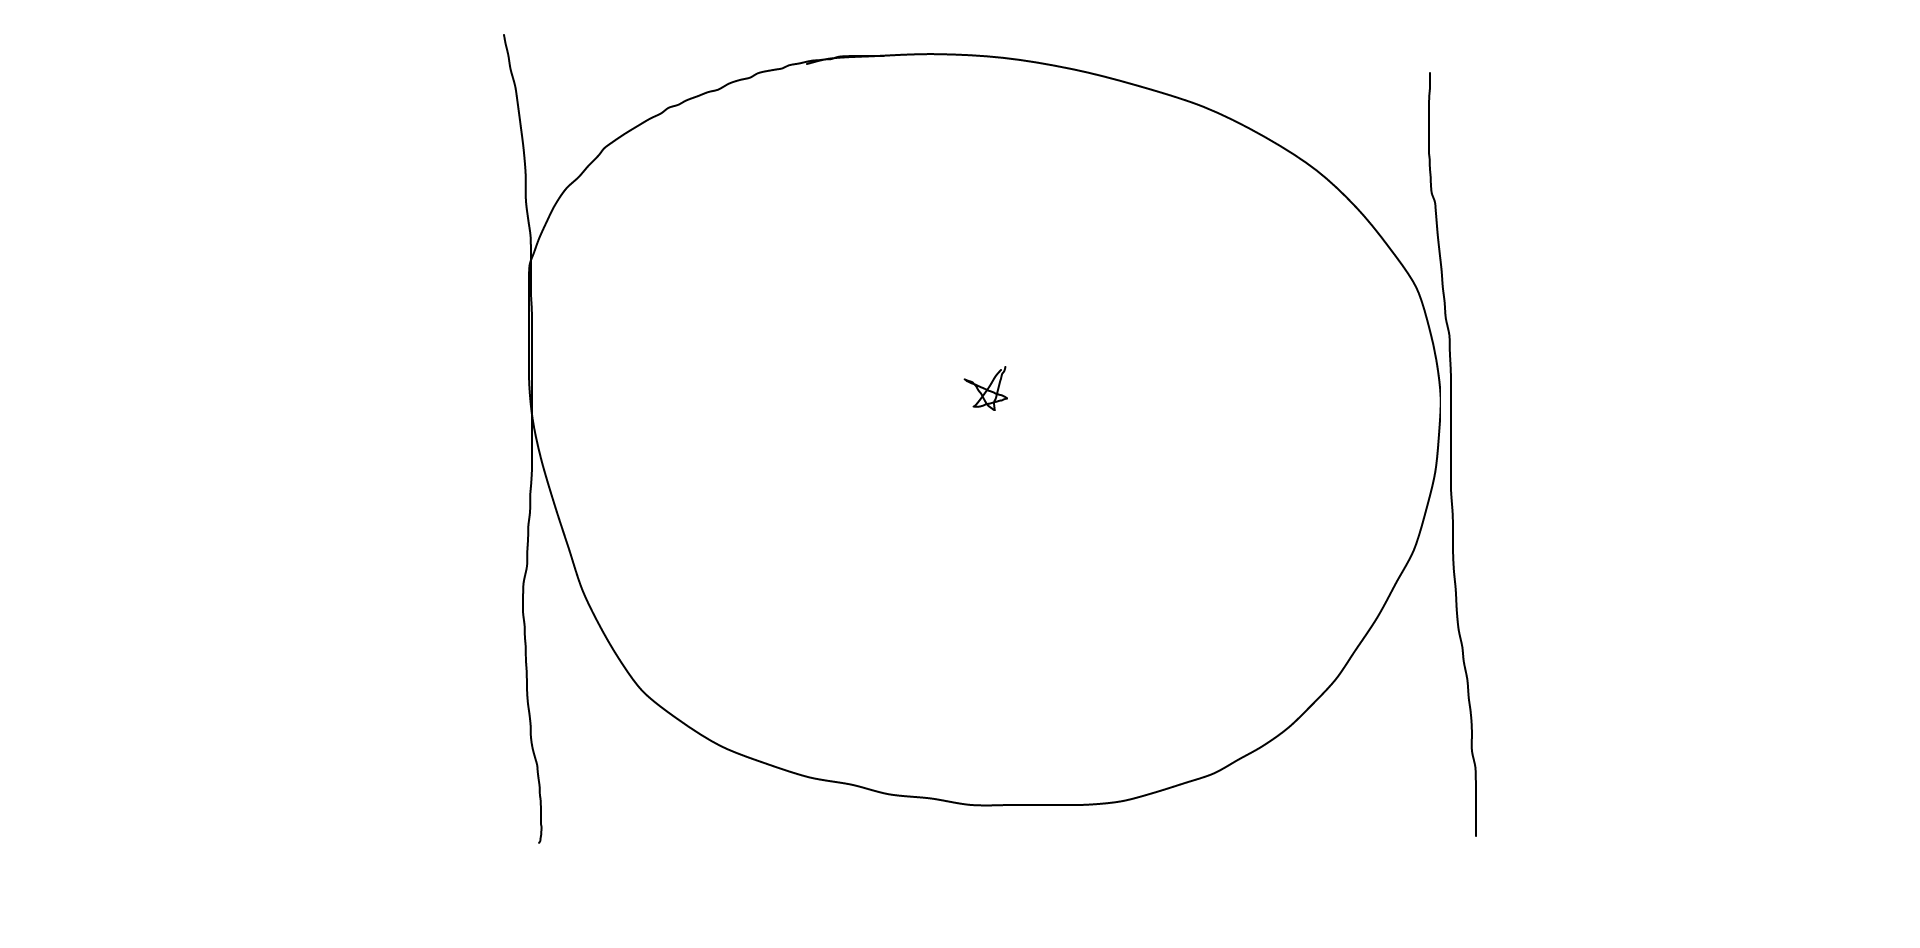
\includegraphics[width=200px]{images/active_regularity.png}
		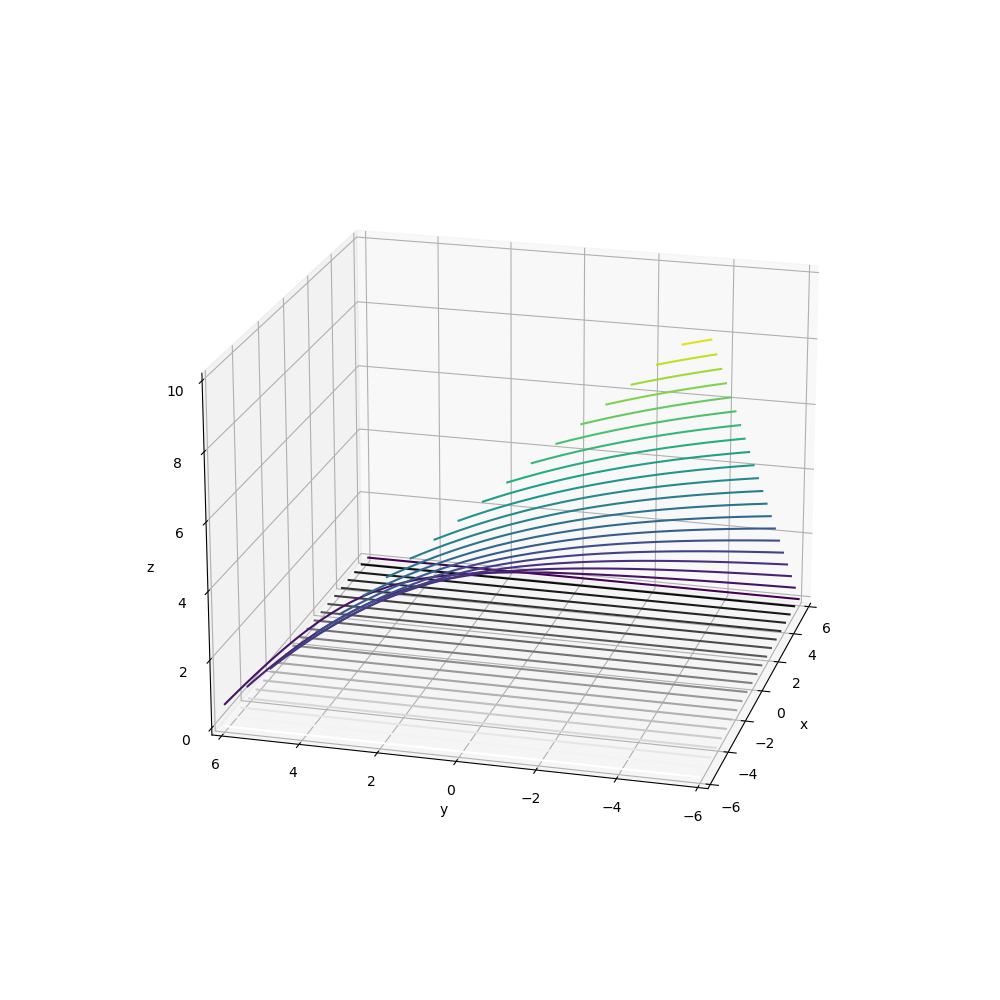
\includegraphics[width=150px]{images/decreasing_regularity.png}
		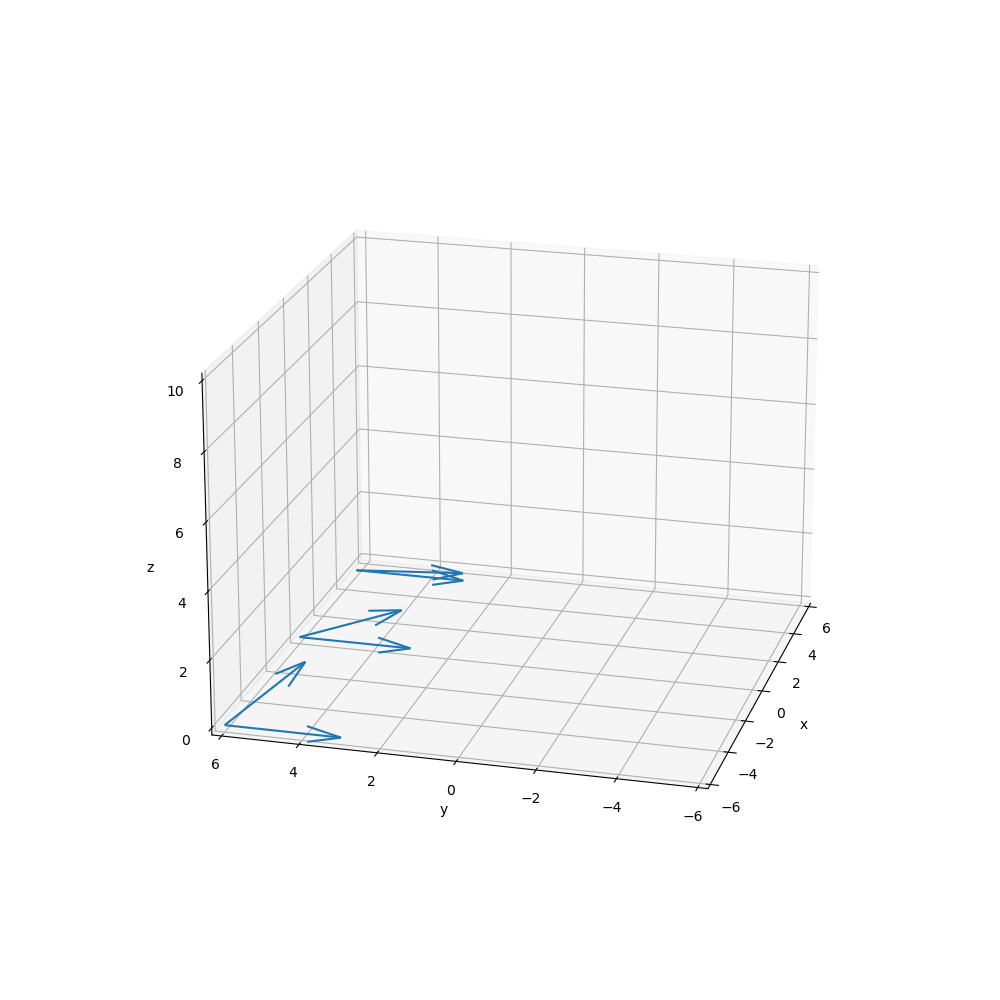
\includegraphics[width=150px]{images/decreasing_regularity_2.png}
	\end{center}
\end{frame}


\begin{frame}{Regularity Assumption}
\begin{itemize}
\item The Mangasarian-Fromovitz constraint qualification requires that for any critical point 
\begin{align*}
\forall x^{\star}, \exists d \in \Rn, \forall i, \\
c_i\left(x^{\star}\right)=0 \wedge \chi\left(x^{\star}\right) = 0 \Longrightarrow \nabla c_i\left(x^{\star}\right)^T d < 0 
\end{align*}
\item We strengthened this qualification:
\begin{align*}
\xout{\forall x \exists d \in \Rn\; \forall i, \nabla c_i\left(x\right)^T d < 0} \\
\xout{\forall x \exists d \in \Rn\; \forall i, \nabla c_i\left(x\right) \approx 0 \Longrightarrow \nabla c_i\left(x\right)^T d < 0} \\
\exists \epsilon>0 \forall x\exists d\in \Rn\; \forall i\; c_i\left(x\right) \approx 0
\Longrightarrow \nabla c_i\left(x\right)^T d < -\epsilon \\
\end{align*}
\end{itemize}
\end{frame}



\begin{frame}{Ellipsoid Recovery}
\begin{itemize}
	\item Given a single feasible point, in general, it can be difficult to find even a second feasible point
	\item This motivates a feasible starting set
	\item For general constraints, we assume a recovery subroutine
	\item For convex constraints, we provide such an algorithm
	\begin{center}
		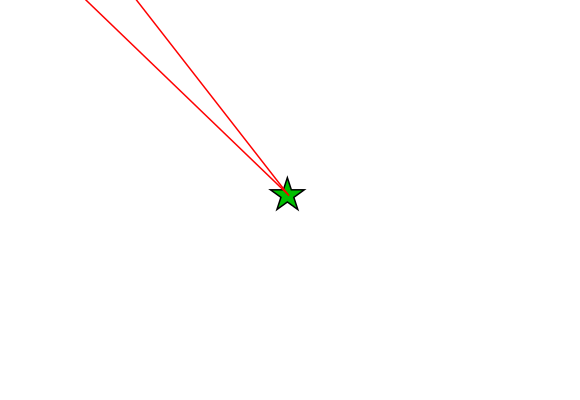
\includegraphics[width=150px]{images/only_one_feasible_point.png}
	\end{center}
\end{itemize}
\end{frame}

\begin{frame}{Convergence Results: The General Case}
\begin{block}{Corollary 4.43}
Suppose that $F_c^{(k)}$ is the true feasible region's linearization at $\xk$.
If $\gamma_{\textrm{min}} = 0$,
\begin{align*}
\liminf_{k\to\infty} \left\|P_{F_c^{(k)}}\left(\xk - \nabla f\left(\xk\right)\right) - \xk\right\| = 0.
\end{align*}
If $\gamma_{\textrm{min}} > 0$,
\begin{align*}
\lim_{k\to\infty} \left\|P_{F_c^{(k)}}\left(\xk - \nabla f\left(\xk\right)\right) - \xk\right\| = 0.
\end{align*}
\end{block}
\end{frame}

\begin{frame}{Convergence Results: The Convex Case}
\begin{block}{Corollary 4.44}
Suppose that the feasible region $F$ is convex. \\
If $\gamma_{\textrm{min}} = 0$,
\begin{align*}
\liminf_{k\to\infty} \left\|P_F\left(\xk - \nabla f\left(\xk\right)\right) - \xk\right\| = 0.
\end{align*}
If $\gamma_{\textrm{min}} > 0$,
\begin{align*}
\lim_{k\to\infty} \left\|P_F\left(\xk - \nabla f\left(\xk\right)\right) - \xk\right\| = 0.
\end{align*}
\end{block}
\end{frame}


\begin{frame}{Numerical Results}
	We compared our algorithm to PDFO, NOMAD, and SCIPY.optimize
	\begin{center}
		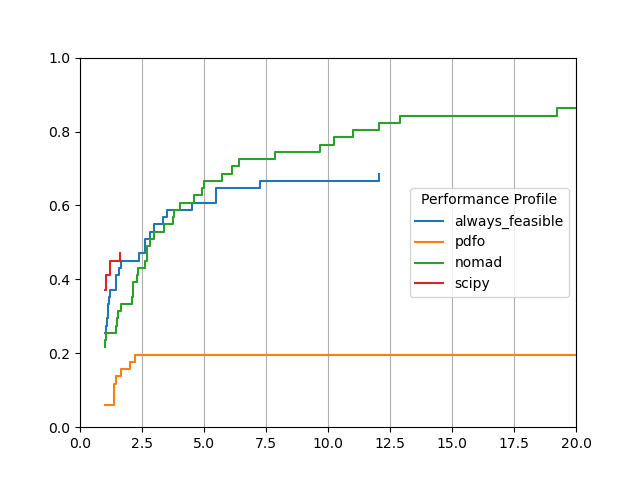
\includegraphics[width=175px]{images/nonlinear_performance_profile.png}
	\end{center}
\end{frame}


% \begin{frame}{Algorithm Variants}
% \begin{itemize}
% 	\item Different forms of the sample region
% 	\item Different forms of the search region
% \end{itemize}
% \end{frame}


\section{Conclusion}

\begin{frame}{Contributions}
	\begin{itemize}
		\setlength\itemsep{1.5em}
		\item First model-based DFO algorithm for non-relaxable constraints
		\item Constructed feasible ellipsoids
		\item Showed sufficient reduction within a buffered region
		\item Convergence in criticality measure
		\item A modified regularity condition
		\item Numerical results with few infeasible evalution attempts
	\end{itemize}
\end{frame}


\frame {
\frametitle{Future Work}
\begin{itemize}
	\setlength\itemsep{2em}
	\item Show error bounds for polyhedral trust regions
	\item Use fewer sample points on narrow constraints
	\item Make assumptions only reference the true constraints
\end{itemize}

}


\frame {
	\frametitle{Questions?}
}

\begin{frame}[allowframebreaks]
	\frametitle{References}
	\bibliographystyle{apalike}
	\bibliography{presentation}
\end{frame}

% 
% \frame {
% \frametitle{Adding Linear Cuts to Feasible Region}
% \begin{itemize}
%	 \item For efficiency, we do not limit the trial point to the inner trust region
%	 \item It is then possible that the trial point found by the trust region subproblem is infeasible
%	 \item If so, we add a constraint that removes this infeasible sample point
%	 \item The program is:
% %		 \begin{itemize}
% %			 \item Start with a polynomial $p$, a tolerance $\epsilon \in (0, 1)$, an set of infeasible points $u_{\text{infe}}^{(j)}$, and a set of feasible points $u_{\text{fe}}^{(i)}$.
%			 \item Compute
%			 \begin{displaymath}
%				 \begin{array}{ccccc}
%	 \min_{s, v^{(j)}, b^{(j)}}   & p(s)			&	   &							\\
%								 & \left(u_{\text{fe}}^{(i)}\right)^T v^{(j)}	 & \le   & b^{(j)}					 \\
%								 & \left(u_{\text{infe}}^{(j)}\right)^T v^{(i)}	  & \ge   & b^{(j)} + \epsilon \Delta_k	   \\
%								 & \|v^{(i)}\|^2   & =	 & 1						   \\
%								 & s		  & \in   & B_{\infty}(x^{(k)}, \Delta_k)	\\
%				 \end{array}
%			 \end{displaymath}
% %		 \end{itemize}
% \end{itemize}
% }
% 
% 
% %								 & I[i]^T v^{(i)}	  & \ge   & \epsilon				\\
% 
% 
% \begin{frame}{Visualizing Linear Cuts}
% \begin{center}
%	 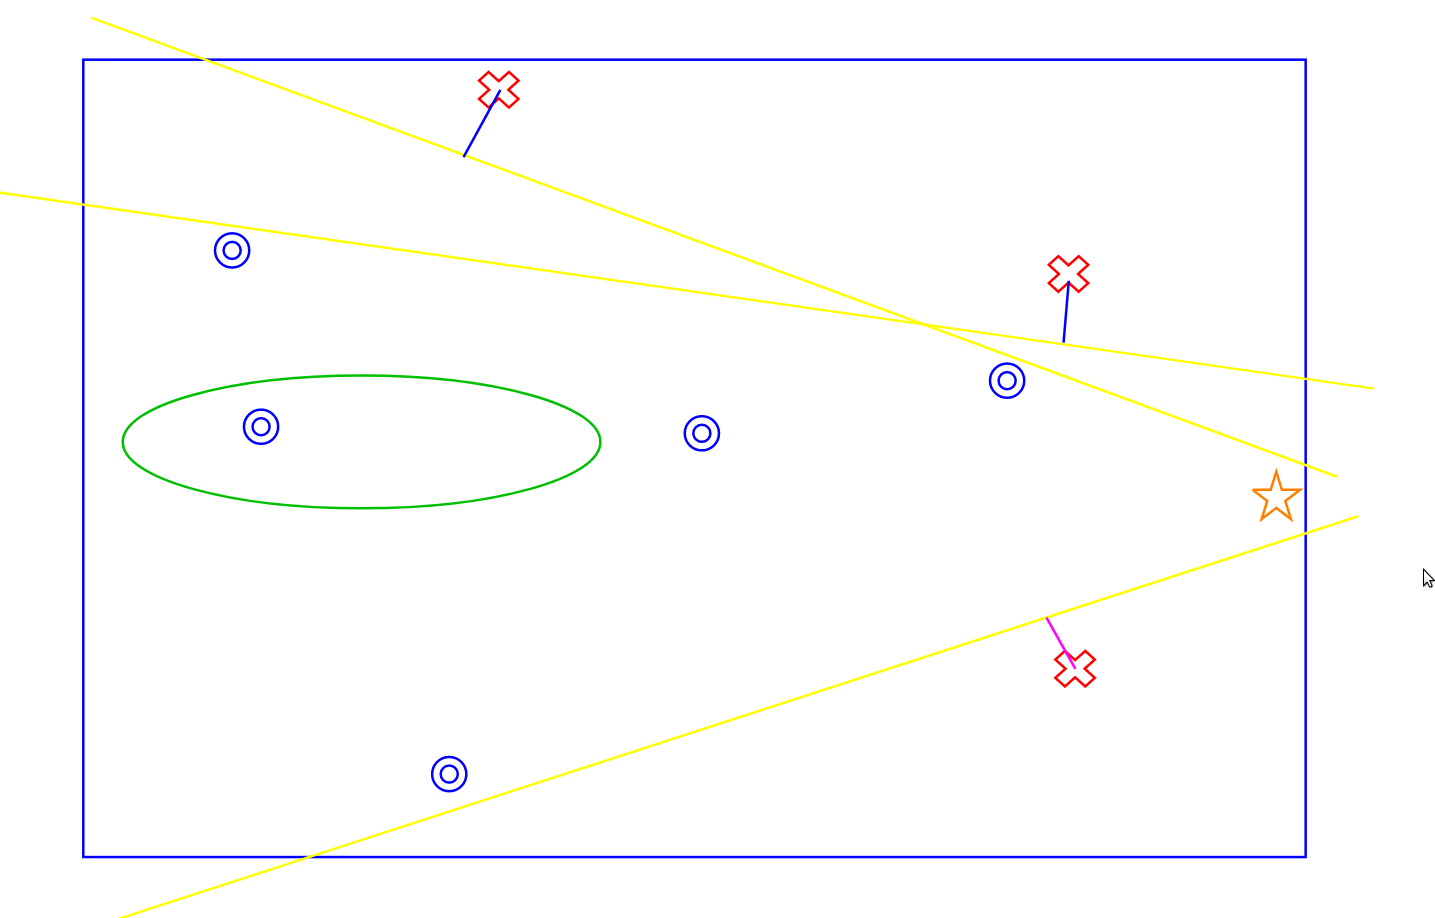
\includegraphics[width=300px]{images/cut_infeasible_points.png}
% \end{center}
% % \includegraphics[width=300px]{images/ellipse_at_current_iterate.png}
% \end{frame}


% 
% 
% \frame{
% \frametitle{Using Fewer Sample Points}
%	 \begin{itemize}
%		 \item With general convex constraints, sufficiently poised sets within the feasible region may not exist.
%		 \item To illustrate, consider finding a fully quadratic model in 2-dimensions.
%		 \item As the constraints become more thin,
%			 \begin{itemize}
%				 \item The model becomes less poised
%				 \item There is less need for requiring the model to be quadratic in $y$.
%			 \end{itemize}
%		 \item We would prefer to use a subset of all quadratics, with fewer points to approximate them.
%	 \end{itemize}
% }
% 
% \frame {
% \frametitle{2D Illustration}
%	 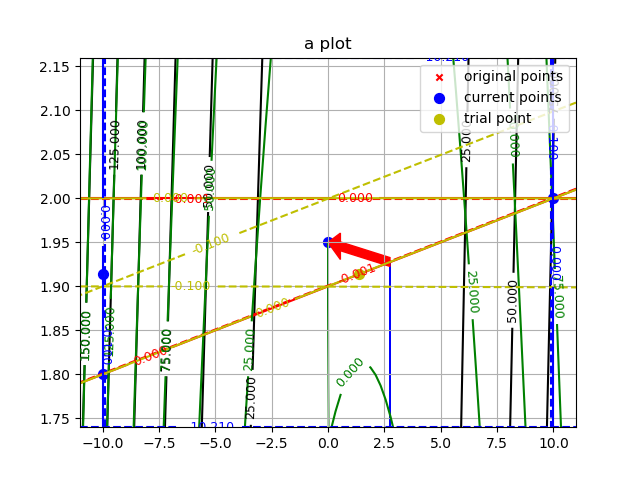
\includegraphics[width=150px]{images/2_2_4_68.png}
%	 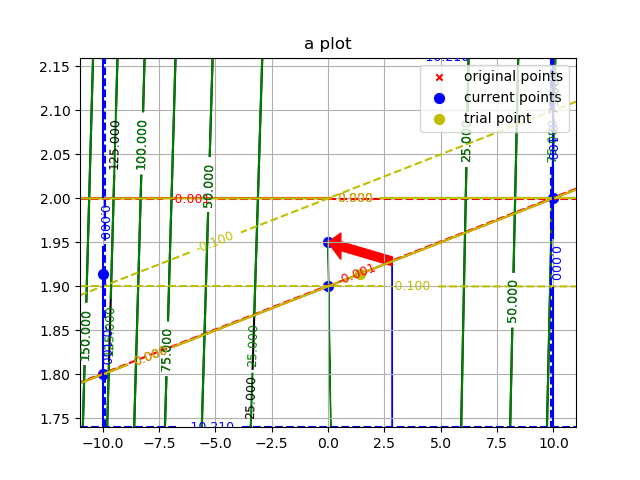
\includegraphics[width=150px]{images/2_3_5_1.png}
% }
% 
% \frame {
% \frametitle{Full pivoting}
%	 \begin{itemize}
%		 \item One approach is to use full pivoting within the LU factorization used compute the Lagrange polynomials.
% 
%		 \item When there are no more pivots greater than a threshold, the LU factorization terminates, and only uses the points and polynomials already computed after zeroing the remaining entries.
%		 
%		 \item This method will provide the next point to use as well as the next polynomial to include.
%		 
%	 \end{itemize}
% }
% 


% Circle





% \begin{frame}{Orders of models}
% 	\begin{itemize}
% 		\item Our algorithm assumes linear models for constraints, and a quadratic model for the objective
% 		\item This is not required, but does introduce the question of how to choose points poised for different orders of models
% 		\item We could select separate points for each different order
% 		\item We could create points for for a quadratic model, and only add points for a linear model if required
% 		\item We could choose points that are best for both models
% 		\item We currently use quadratic models for both
% 	\end{itemize}
% \end{frame}


\end{document}
